% Options for packages loaded elsewhere
% Options for packages loaded elsewhere
\PassOptionsToPackage{unicode}{hyperref}
\PassOptionsToPackage{hyphens}{url}
\PassOptionsToPackage{space}{xeCJK}
%
\documentclass[
  Letterpaper,
]{scrbook}
\usepackage{xcolor}
\usepackage[paperwidth=6in,paperheight=9in]{geometry}
\usepackage{amsmath,amssymb}
\setcounter{secnumdepth}{5}
\usepackage{iftex}
\ifPDFTeX
  \usepackage[T1]{fontenc}
  \usepackage[utf8]{inputenc}
  \usepackage{textcomp} % provide euro and other symbols
\else % if luatex or xetex
  \usepackage{unicode-math} % this also loads fontspec
  \defaultfontfeatures{Scale=MatchLowercase}
  \defaultfontfeatures[\rmfamily]{Ligatures=TeX,Scale=1}
\fi
\usepackage{lmodern}
\ifPDFTeX\else
  % xetex/luatex font selection
  \setmainfont[]{Georgia}
  \ifXeTeX
    \usepackage{xeCJK}
    \setCJKmainfont[]{STSong}
  \fi
  \ifLuaTeX
    \usepackage[]{luatexja-fontspec}
    \setmainjfont[]{STSong}
  \fi
\fi
% Use upquote if available, for straight quotes in verbatim environments
\IfFileExists{upquote.sty}{\usepackage{upquote}}{}
\IfFileExists{microtype.sty}{% use microtype if available
  \usepackage[]{microtype}
  \UseMicrotypeSet[protrusion]{basicmath} % disable protrusion for tt fonts
}{}
\makeatletter
\@ifundefined{KOMAClassName}{% if non-KOMA class
  \IfFileExists{parskip.sty}{%
    \usepackage{parskip}
  }{% else
    \setlength{\parindent}{0pt}
    \setlength{\parskip}{6pt plus 2pt minus 1pt}}
}{% if KOMA class
  \KOMAoptions{parskip=half}}
\makeatother
% Make \paragraph and \subparagraph free-standing
\makeatletter
\ifx\paragraph\undefined\else
  \let\oldparagraph\paragraph
  \renewcommand{\paragraph}{
    \@ifstar
      \xxxParagraphStar
      \xxxParagraphNoStar
  }
  \newcommand{\xxxParagraphStar}[1]{\oldparagraph*{#1}\mbox{}}
  \newcommand{\xxxParagraphNoStar}[1]{\oldparagraph{#1}\mbox{}}
\fi
\ifx\subparagraph\undefined\else
  \let\oldsubparagraph\subparagraph
  \renewcommand{\subparagraph}{
    \@ifstar
      \xxxSubParagraphStar
      \xxxSubParagraphNoStar
  }
  \newcommand{\xxxSubParagraphStar}[1]{\oldsubparagraph*{#1}\mbox{}}
  \newcommand{\xxxSubParagraphNoStar}[1]{\oldsubparagraph{#1}\mbox{}}
\fi
\makeatother

\usepackage{color}
\usepackage{fancyvrb}
\newcommand{\VerbBar}{|}
\newcommand{\VERB}{\Verb[commandchars=\\\{\}]}
\DefineVerbatimEnvironment{Highlighting}{Verbatim}{commandchars=\\\{\}}
% Add ',fontsize=\small' for more characters per line
\usepackage{framed}
\definecolor{shadecolor}{RGB}{241,243,245}
\newenvironment{Shaded}{\begin{snugshade}}{\end{snugshade}}
\newcommand{\AlertTok}[1]{\textcolor[rgb]{0.68,0.00,0.00}{#1}}
\newcommand{\AnnotationTok}[1]{\textcolor[rgb]{0.37,0.37,0.37}{#1}}
\newcommand{\AttributeTok}[1]{\textcolor[rgb]{0.40,0.45,0.13}{#1}}
\newcommand{\BaseNTok}[1]{\textcolor[rgb]{0.68,0.00,0.00}{#1}}
\newcommand{\BuiltInTok}[1]{\textcolor[rgb]{0.00,0.23,0.31}{#1}}
\newcommand{\CharTok}[1]{\textcolor[rgb]{0.13,0.47,0.30}{#1}}
\newcommand{\CommentTok}[1]{\textcolor[rgb]{0.37,0.37,0.37}{#1}}
\newcommand{\CommentVarTok}[1]{\textcolor[rgb]{0.37,0.37,0.37}{\textit{#1}}}
\newcommand{\ConstantTok}[1]{\textcolor[rgb]{0.56,0.35,0.01}{#1}}
\newcommand{\ControlFlowTok}[1]{\textcolor[rgb]{0.00,0.23,0.31}{\textbf{#1}}}
\newcommand{\DataTypeTok}[1]{\textcolor[rgb]{0.68,0.00,0.00}{#1}}
\newcommand{\DecValTok}[1]{\textcolor[rgb]{0.68,0.00,0.00}{#1}}
\newcommand{\DocumentationTok}[1]{\textcolor[rgb]{0.37,0.37,0.37}{\textit{#1}}}
\newcommand{\ErrorTok}[1]{\textcolor[rgb]{0.68,0.00,0.00}{#1}}
\newcommand{\ExtensionTok}[1]{\textcolor[rgb]{0.00,0.23,0.31}{#1}}
\newcommand{\FloatTok}[1]{\textcolor[rgb]{0.68,0.00,0.00}{#1}}
\newcommand{\FunctionTok}[1]{\textcolor[rgb]{0.28,0.35,0.67}{#1}}
\newcommand{\ImportTok}[1]{\textcolor[rgb]{0.00,0.46,0.62}{#1}}
\newcommand{\InformationTok}[1]{\textcolor[rgb]{0.37,0.37,0.37}{#1}}
\newcommand{\KeywordTok}[1]{\textcolor[rgb]{0.00,0.23,0.31}{\textbf{#1}}}
\newcommand{\NormalTok}[1]{\textcolor[rgb]{0.00,0.23,0.31}{#1}}
\newcommand{\OperatorTok}[1]{\textcolor[rgb]{0.37,0.37,0.37}{#1}}
\newcommand{\OtherTok}[1]{\textcolor[rgb]{0.00,0.23,0.31}{#1}}
\newcommand{\PreprocessorTok}[1]{\textcolor[rgb]{0.68,0.00,0.00}{#1}}
\newcommand{\RegionMarkerTok}[1]{\textcolor[rgb]{0.00,0.23,0.31}{#1}}
\newcommand{\SpecialCharTok}[1]{\textcolor[rgb]{0.37,0.37,0.37}{#1}}
\newcommand{\SpecialStringTok}[1]{\textcolor[rgb]{0.13,0.47,0.30}{#1}}
\newcommand{\StringTok}[1]{\textcolor[rgb]{0.13,0.47,0.30}{#1}}
\newcommand{\VariableTok}[1]{\textcolor[rgb]{0.07,0.07,0.07}{#1}}
\newcommand{\VerbatimStringTok}[1]{\textcolor[rgb]{0.13,0.47,0.30}{#1}}
\newcommand{\WarningTok}[1]{\textcolor[rgb]{0.37,0.37,0.37}{\textit{#1}}}

\usepackage{longtable,booktabs,array}
\usepackage{calc} % for calculating minipage widths
% Correct order of tables after \paragraph or \subparagraph
\usepackage{etoolbox}
\makeatletter
\patchcmd\longtable{\par}{\if@noskipsec\mbox{}\fi\par}{}{}
\makeatother
% Allow footnotes in longtable head/foot
\IfFileExists{footnotehyper.sty}{\usepackage{footnotehyper}}{\usepackage{footnote}}
\makesavenoteenv{longtable}
\usepackage{graphicx}
\makeatletter
\newsavebox\pandoc@box
\newcommand*\pandocbounded[1]{% scales image to fit in text height/width
  \sbox\pandoc@box{#1}%
  \Gscale@div\@tempa{\textheight}{\dimexpr\ht\pandoc@box+\dp\pandoc@box\relax}%
  \Gscale@div\@tempb{\linewidth}{\wd\pandoc@box}%
  \ifdim\@tempb\p@<\@tempa\p@\let\@tempa\@tempb\fi% select the smaller of both
  \ifdim\@tempa\p@<\p@\scalebox{\@tempa}{\usebox\pandoc@box}%
  \else\usebox{\pandoc@box}%
  \fi%
}
% Set default figure placement to htbp
\def\fps@figure{htbp}
\makeatother


% definitions for citeproc citations
\NewDocumentCommand\citeproctext{}{}
\NewDocumentCommand\citeproc{mm}{%
  \begingroup\def\citeproctext{#2}\cite{#1}\endgroup}
\makeatletter
 % allow citations to break across lines
 \let\@cite@ofmt\@firstofone
 % avoid brackets around text for \cite:
 \def\@biblabel#1{}
 \def\@cite#1#2{{#1\if@tempswa , #2\fi}}
\makeatother
\newlength{\cslhangindent}
\setlength{\cslhangindent}{1.5em}
\newlength{\csllabelwidth}
\setlength{\csllabelwidth}{3em}
\newenvironment{CSLReferences}[2] % #1 hanging-indent, #2 entry-spacing
 {\begin{list}{}{%
  \setlength{\itemindent}{0pt}
  \setlength{\leftmargin}{0pt}
  \setlength{\parsep}{0pt}
  % turn on hanging indent if param 1 is 1
  \ifodd #1
   \setlength{\leftmargin}{\cslhangindent}
   \setlength{\itemindent}{-1\cslhangindent}
  \fi
  % set entry spacing
  \setlength{\itemsep}{#2\baselineskip}}}
 {\end{list}}
\usepackage{calc}
\newcommand{\CSLBlock}[1]{\hfill\break\parbox[t]{\linewidth}{\strut\ignorespaces#1\strut}}
\newcommand{\CSLLeftMargin}[1]{\parbox[t]{\csllabelwidth}{\strut#1\strut}}
\newcommand{\CSLRightInline}[1]{\parbox[t]{\linewidth - \csllabelwidth}{\strut#1\strut}}
\newcommand{\CSLIndent}[1]{\hspace{\cslhangindent}#1}



\setlength{\emergencystretch}{3em} % prevent overfull lines

\providecommand{\tightlist}{%
  \setlength{\itemsep}{0pt}\setlength{\parskip}{0pt}}



 


\usepackage{xeCJK}
\setCJKmainfont{STSong}
\raggedbottom
\makeatletter
\@ifpackageloaded{tcolorbox}{}{\usepackage[skins,breakable]{tcolorbox}}
\@ifpackageloaded{fontawesome5}{}{\usepackage{fontawesome5}}
\definecolor{quarto-callout-color}{HTML}{909090}
\definecolor{quarto-callout-note-color}{HTML}{0758E5}
\definecolor{quarto-callout-important-color}{HTML}{CC1914}
\definecolor{quarto-callout-warning-color}{HTML}{EB9113}
\definecolor{quarto-callout-tip-color}{HTML}{00A047}
\definecolor{quarto-callout-caution-color}{HTML}{FC5300}
\definecolor{quarto-callout-color-frame}{HTML}{acacac}
\definecolor{quarto-callout-note-color-frame}{HTML}{4582ec}
\definecolor{quarto-callout-important-color-frame}{HTML}{d9534f}
\definecolor{quarto-callout-warning-color-frame}{HTML}{f0ad4e}
\definecolor{quarto-callout-tip-color-frame}{HTML}{02b875}
\definecolor{quarto-callout-caution-color-frame}{HTML}{fd7e14}
\makeatother
\makeatletter
\@ifpackageloaded{bookmark}{}{\usepackage{bookmark}}
\makeatother
\makeatletter
\@ifpackageloaded{caption}{}{\usepackage{caption}}
\AtBeginDocument{%
\ifdefined\contentsname
  \renewcommand*\contentsname{Table of contents}
\else
  \newcommand\contentsname{Table of contents}
\fi
\ifdefined\listfigurename
  \renewcommand*\listfigurename{List of Figures}
\else
  \newcommand\listfigurename{List of Figures}
\fi
\ifdefined\listtablename
  \renewcommand*\listtablename{List of Tables}
\else
  \newcommand\listtablename{List of Tables}
\fi
\ifdefined\figurename
  \renewcommand*\figurename{Figure}
\else
  \newcommand\figurename{Figure}
\fi
\ifdefined\tablename
  \renewcommand*\tablename{Table}
\else
  \newcommand\tablename{Table}
\fi
}
\@ifpackageloaded{float}{}{\usepackage{float}}
\floatstyle{ruled}
\@ifundefined{c@chapter}{\newfloat{codelisting}{h}{lop}}{\newfloat{codelisting}{h}{lop}[chapter]}
\floatname{codelisting}{Listing}
\newcommand*\listoflistings{\listof{codelisting}{List of Listings}}
\makeatother
\makeatletter
\makeatother
\makeatletter
\@ifpackageloaded{caption}{}{\usepackage{caption}}
\@ifpackageloaded{subcaption}{}{\usepackage{subcaption}}
\makeatother
\usepackage{bookmark}
\IfFileExists{xurl.sty}{\usepackage{xurl}}{} % add URL line breaks if available
\urlstyle{same}
\hypersetup{
  pdftitle={鏈上商業解決方案},
  pdfauthor={孫波 (Apollo Sun)},
  hidelinks,
  pdfcreator={LaTeX via pandoc}}


\title{鏈上商業解決方案}
\author{孫波 (Apollo Sun)}
\date{2025-07-28}
\begin{document}
\frontmatter
\maketitle

\renewcommand*\contentsname{Table of contents}
{
\setcounter{tocdepth}{1}
\tableofcontents
}

\mainmatter
\bookmarksetup{startatroot}

\chapter*{前言}\label{ux524dux8a00}
\addcontentsline{toc}{chapter}{前言}

\markboth{前言}{前言}

\textbf{鏈上商業:第三次商業革命}

在過去的商業世界裡,「賺錢」等於「賺利潤」。但是在鏈上商業時代,「賺錢」等於「賺流通」。我們發現,真正讓人們富有的不是把錢儲存起來,而是把錢用在能產生價值交換的地方。「花得越多,賺得越多」的概念不是白日夢,而是建立在區塊鏈技術和去中心化商業邏輯上的現實可能。

\section*{新商業文明的基礎}\label{ux65b0ux5546ux696dux6587ux660eux7684ux57faux790e}
\addcontentsline{toc}{section}{新商業文明的基礎}

\markright{新商業文明的基礎}

鏈上商業代表了一個全新的商業文明------不是一個單一的平臺,而是一個以價值共享、去中介化和信任重構為中心的商業生態系統。它不依賴於任何單一國家或公司,也不以廣告投放為中心,而是建立在社區參與和利益共創的基礎上。

鏈上商業的出現不是為了對抗傳統,而是為了解決傳統商業系統中長期存在的痛點:

\begin{itemize}
\tightlist
\item
  為什麼越來越多商家的利潤被平臺消耗?
\item
  為什麼增加廣告支出不能帶來忠實用戶?
\item
  為什麼消費者忠誠度不能轉化為任何回報?
\end{itemize}

這些問題不是偶然的------它們源於我們商業設計中的結構性問題。鏈上商業為這些核心問題提供了一個可部署的解決方案。

\section*{從「賺錢」到「賺流通」}\label{ux5f9eux8cfaux9322ux5230ux8cfaux6d41ux901a}
\addcontentsline{toc}{section}{從「賺錢」到「賺流通」}

\markright{從「賺錢」到「賺流通」}

什麼是「財富」?在農業時代,是土地。在工業時代,是資本和工廠。在數位時代,變成了流量和注意力。但無論時代如何變化,有一個不變的常數:真正的財富來自「流動」。

傳統的經濟邏輯教我們儲蓄------將收入轉化為銀行存款或房地產資產,以確保未來的安全。然而,在通脹壓力和貨幣超發的情況下,儲蓄的購買力每年都在下降。真正帶來升值的是流動性。

當資本停滯時,就等於損失。當資本通過流通創造價值時,它不僅不會縮水,還能帶來複合回報。這就是「賺流通」的本質邏輯------不是儲存,而是讓錢在正確的生態系統中流動、創造和重新分配。

\section*{信任的演變:從黃金到社區共識}\label{ux4fe1ux4efbux7684ux6f14ux8b8aux5f9eux9ec3ux91d1ux5230ux793eux5340ux5171ux8b58}
\addcontentsline{toc}{section}{信任的演變:從黃金到社區共識}

\markright{信任的演變:從黃金到社區共識}

貨幣的演變其實是「信任憑證」的演變:

\begin{itemize}
\tightlist
\item
  \textbf{黃金時代}:對貨幣的信任來自實物資產
\item
  \textbf{紙幣時代}:信任轉移到國家和央行
\item
  \textbf{數位貨幣時代}:信任建立在算法、共識機制和社區上
\end{itemize}

比特幣和以太坊的成功證明,人們已經開始相信「去中心化」系統可以維持公平透明的價值交換,而不被任何單一實體操控。這為鏈上商業出現提供了信任的技術基礎。

\section*{Web3:重構商業規則}\label{web3ux91cdux69cbux5546ux696dux898fux5247}
\addcontentsline{toc}{section}{Web3:重構商業規則}

\markright{Web3:重構商業規則}

Web3代表了下一代網際網路,但真正改變商業規則的不僅僅是技術------而是權力結構和價值分配方式的重構。

傳統商業邏輯是「中心化的」:數據屬於平臺,用戶只是數據生產者,價值被平臺捕獲,參與者不能分享利潤。規則由平臺制定,商家和用戶只能接受。

Web3提出了顛覆性邏輯:用戶擁有數據,社區共治生態系統,價值增長共享。

這種價值主權讓用戶真正「擁有自己的經濟系統」,迫使平臺重新考慮與參與者的關係。通過透明規則、自動執行和公平分配機制,鏈上商業消除了傳統中介剝削,同時創造可持續的價值增長。

\section*{鏈上商業的六大支柱}\label{ux93c8ux4e0aux5546ux696dux7684ux516dux5927ux652fux67f1}
\addcontentsline{toc}{section}{鏈上商業的六大支柱}

\markright{鏈上商業的六大支柱}

鏈上商業系統能夠實現實施、擴展和可持續發展,因為其核心在於制度設計------一個由六大支柱組成的商業運營模式:

\begin{enumerate}
\def\labelenumi{\arabic{enumi}.}
\tightlist
\item
  \textbf{公平利潤分享機制} - 每筆交易自動分配收益
\item
  \textbf{穩定代幣價值支撐模型} - 真實交易支撐,而非投機
\item
  \textbf{可擴展的商家成長階梯} - 從個人創作者到區域網路
\item
  \textbf{高信任社區網路} - 網路節點,而非金字塔結構
\item
  \textbf{真正的「共享」利潤分配} - 用戶是節點,而非成員
\item
  \textbf{高頻次必需場景} - 真實商業,而非概念
\end{enumerate}

這代表了一個可以自我運營、自我擴展、自我升值的商業生態系統,而不是任何公司的「平臺系統」。

\section*{屬於每個人的革命}\label{ux5c6cux65bcux6bcfux500bux4ebaux7684ux9769ux547d}
\addcontentsline{toc}{section}{屬於每個人的革命}

\markright{屬於每個人的革命}

鏈上商業正在發起一場真正屬於「每個人」的革命。在這場革命中,你不需要背景或大資本------你只需要行動、參與和貢獻。

本書將逐步揭示鏈上商業的出現、運營邏輯、制度設計和全球擴張模式。更重要的是,我希望它能幫助你打開一個全新的視角:在未來,不了解鏈上商業就像25年前不了解網際網路一樣。

在未來的商業世界中,流通比擁有更重要。我們站在真正商業革命的門檻上。而你將不再只是參與者------你是這場革命中的一個節點。

\begin{tcolorbox}[enhanced jigsaw, toptitle=1mm, breakable, bottomtitle=1mm, arc=.35mm, title=\textcolor{quarto-callout-note-color}{\faInfo}\hspace{0.5em}{關於本書}, opacitybacktitle=0.6, left=2mm, toprule=.15mm, colframe=quarto-callout-note-color-frame, opacityback=0, bottomrule=.15mm, rightrule=.15mm, titlerule=0mm, leftrule=.75mm, colbacktitle=quarto-callout-note-color!10!white, colback=white, coltitle=black]

本書使用 Proofbound CC 模板 CLI 工具創建。了解更多關於 Proofbound
的信息,請訪問 \url{https://proofbound.com}。

\end{tcolorbox}

\part{第一部分:基礎革命}

\chapter{第一章:从赚钱到赚流通}\label{sec-earning-circulation}

\section{传统商业的局限性}\label{ux4f20ux7edfux5546ux4e1aux7684ux5c40ux9650ux6027}

在传统商业模式中,``赚钱''的定义很简单:收入减去成本等于利润。这种线性思维模式主导了几个世纪的商业实践,但在数字化时代显露出了根本性的缺陷。

\subsection{储蓄悖论}\label{ux50a8ux84c4ux6096ux8bba}

传统经济学教导我们储蓄的重要性------将收入的一部分存起来,以备不时之需。然而,在当今的经济环境下,这种策略面临着严重的挑战:

\begin{enumerate}
\def\labelenumi{\arabic{enumi}.}
\tightlist
\item
  \textbf{通胀侵蚀}:持续的通胀使储蓄的购买力每年递减
\item
  \textbf{机会成本}:静态资金失去了参与价值创造的机会
\item
  \textbf{流动性陷阱}:过度储蓄导致经济活力下降
\end{enumerate}

\subsection{中介剥削}\label{ux4e2dux4ecbux5265ux524a}

传统商业生态中,价值创造者往往不是最大的受益者:

\begin{itemize}
\tightlist
\item
  商家的利润被平台抽取
\item
  消费者的数据被无偿收集
\item
  创作者的内容被平台变现
\end{itemize}

\section{链上商业的流通逻辑}\label{ux94feux4e0aux5546ux4e1aux7684ux6d41ux901aux903bux8f91}

链上商业提出了一个革命性的概念:\textbf{财富不是储存的结果,而是流通的产物}。

\subsection{流通即价值}\label{ux6d41ux901aux5373ux4ef7ux503c}

在链上商业生态中:

\begin{enumerate}
\def\labelenumi{\arabic{enumi}.}
\tightlist
\item
  \textbf{每次交易都创造价值}:不是零和游戏,而是正和游戏
\item
  \textbf{参与即获得}:用户的每个行为都能获得相应的回报
\item
  \textbf{网络效应放大}:参与者越多,个体收益越大
\end{enumerate}

\subsection{复合增长机制}\label{ux590dux5408ux589eux957fux673aux5236}

通过智能合约和代币经济学,链上商业实现了:

\begin{itemize}
\tightlist
\item
  自动化的价值分配
\item
  透明的收益计算
\item
  去中心化的治理机构
\end{itemize}

\section{实践案例:从概念到现实}\label{ux5b9eux8df5ux6848ux4f8bux4eceux6982ux5ff5ux5230ux73b0ux5b9e}

\subsection{案例一:社区驱动的电商平台}\label{ux6848ux4f8bux4e00ux793eux533aux9a71ux52a8ux7684ux7535ux5546ux5e73ux53f0}

传统电商平台模式: - 商家缴纳入驻费用 - 平台抽取交易佣金 -
消费者仅获得商品,无其他收益

链上商业模式: - 商家通过代币质押参与 - 交易产生的价值按贡献分配 -
消费者获得代币奖励,形成复购激励

\subsection{案例二:内容创作生态}\label{ux6848ux4f8bux4e8cux5185ux5bb9ux521bux4f5cux751fux6001}

传统模式的问题: - 创作者依赖平台算法 - 收益分配不透明 -
用户数据被平台垄断

链上商业解决方案: - 创作者直接获得用户支持 - 智能合约保证收益分配 -
用户拥有数据主权

\section{技术实现框架}\label{ux6280ux672fux5b9eux73b0ux6846ux67b6}

\subsection{智能合约架构}\label{ux667aux80fdux5408ux7ea6ux67b6ux6784}

\begin{Shaded}
\begin{Highlighting}[]
\NormalTok{contract CirculationReward \{}
\NormalTok{    mapping(address =\textgreater{} uint256) public contributions;}
\NormalTok{    mapping(address =\textgreater{} uint256) public rewards;}
    
\NormalTok{    function contribute() external payable \{}
\NormalTok{        contributions[msg.sender] += msg.value;}
\NormalTok{        calculateRewards();}
\NormalTok{    \}}
    
\NormalTok{    function calculateRewards() internal \{}
\NormalTok{        // 基于贡献和网络效应的奖励计算}
\NormalTok{    \}}
\NormalTok{\}}
\end{Highlighting}
\end{Shaded}

\subsection{代币经济模型}\label{ux4ee3ux5e01ux7ecfux6d4eux6a21ux578b}

\begin{enumerate}
\def\labelenumi{\arabic{enumi}.}
\tightlist
\item
  \textbf{流通激励}:持有者通过使用代币获得奖励
\item
  \textbf{网络价值}:代币价值与网络活跃度正相关
\item
  \textbf{治理权益}:代币持有者参与生态治理
\end{enumerate}

\section{从理论到实践的路径}\label{ux4eceux7406ux8bbaux5230ux5b9eux8df5ux7684ux8defux5f84}

\subsection{第一阶段:建立基础设施}\label{ux7b2cux4e00ux9636ux6bb5ux5efaux7acbux57faux7840ux8bbeux65bd}

\begin{itemize}
\tightlist
\item
  部署智能合约
\item
  建立用户界面
\item
  构建初始社区
\end{itemize}

\subsection{第二阶段:扩展网络效应}\label{ux7b2cux4e8cux9636ux6bb5ux6269ux5c55ux7f51ux7edcux6548ux5e94}

\begin{itemize}
\tightlist
\item
  吸引更多参与者
\item
  优化激励机制
\item
  建立信任体系
\end{itemize}

\subsection{第三阶段:生态自治}\label{ux7b2cux4e09ux9636ux6bb5ux751fux6001ux81eaux6cbb}

\begin{itemize}
\tightlist
\item
  社区自主治理
\item
  持续价值创造
\item
  全球网络扩张
\end{itemize}

\section{结论}\label{ux7ed3ux8bba}

从''赚钱''到''赚流通''的转变不仅是概念上的革新,更是商业模式的根本性变革。通过区块链技术和去中心化治理,我们能够构建一个真正服务于参与者的商业生态系统。

在下一章中,我们将深入探讨Web3如何重构传统商业规则,以及这种重构对整个商业生态的深远影响。

\chapter{第二章:Web3的商业颠覆}\label{sec-web3-disruption}

去中心化技术如何重写商业规则

Web3的出现远不止是对现有互联网基础设施的技术升级。从根本上说,Web3彻底重构了平台、用户和价值创造之间的关系,以挑战现代商业活动基本假设的方式。虽然Web2将权力和利润集中在平台所有者手中,但Web3在数字生态系统的所有参与者之间分配权威和经济利益。

这种转变超越了简单的技术改进,涵盖了对数字环境中商业关系如何运作的完全重新思考。传统平台从用户互动和商家活动中提取价值,而Web3系统创建了在所有网络效应贡献者之间共享价值的机制。其影响延伸到现代商业的每个方面,从企业如何获取客户到个人如何将其数字活动货币化。

要理解这种颠覆,需要检查的不仅是Web3技术能做什么,还要看为什么它们代表了超越中心化平台经济中出现的限制和矛盾的必要进化。目前约束企业和消费者的平台陷阱创造了Web3架构独特定位来解决的系统性低效。

\section{平台陷阱}\label{ux5e73ux53f0ux9677ux9631}

当代数字商业通过中心化平台运营,这些平台逐渐集中了对市场准入、客户关系和价值分配的巨大权力。这些平台最初通过提供有价值的服务吸引参与者:亚马逊为卖家提供市场准入,为买家提供便利;谷歌提供免费搜索和广告工具;Facebook跨越地理界限连接人们。然而,随着这些平台实现市场主导地位,它们的激励从服务参与者转向从其中介地位提取最大价值。

平台经济学的数学结构在平台所有者和其他参与者之间创造了固有冲突。平台通过捕获流经其系统的交易、广告支出或订阅费用的百分比来产生收入。这创造了最大化通过平台流动的价值量同时增加平台所有者捕获百分比的压力。结果是对商家和消费者的逐渐挤压,因为平台为了自己的盈利能力而不是生态系统健康进行优化。

考虑亚马逊与第三方卖家关系的演变。最初,亚马逊收取适度费用并提供真正帮助商家接触新客户的有价值服务。然而,随着时间推移,平台引入了日益复杂的费用结构、强制广告要求和限制性政策,有效地迫使商家交出更大部分的收入来维持市场准入。在平台上取得成功的商家经常发现自己被困:他们无法承担离开,因为亚马逊代表了他们销售的如此大部分,但他们无法实现可持续盈利,因为亚马逊的费用消耗了他们的大部分利润率。

这种动态超越了个别交易,涵盖了数据所有权和客户关系。平台商家无法访问详细的客户信息,无法与买家建立直接关系,无法将其客户群转移到替代平台。平台拥有所有客户数据和关系,利用这种信息不对称来维持对市场准入的控制。商家变得依赖于平台的算法、广告系统和政策决定,当这些系统以损害其业务的方式改变时,几乎没有追索权。

平台陷阱也影响消费者,尽管通常以不太明显的方式。虽然平台提供便利和选择,但它们也创造了过滤泡沫,通过算法推荐操纵购买决策,并随着实现市场主导地位逐渐提高价格。消费者通过与平台的互动产生有价值的数据,但却没有收到这种价值创造的补偿。相反,他们的数据被出售给广告商,并用于优化从他们钱包中提取资金。

也许最重要的是,平台模式在生态系统发展和参与者成功方面造成了系统性投资不足。由于平台从其中介地位而不是从生态系统参与者的成功中获利,它们在帮助商家改善业务或为消费者提供真正最优结果方面的激励有限。平台的利益与维持依赖性和提取价值一致,而不是为参与者之间的广泛繁荣创造条件。

\pandocbounded{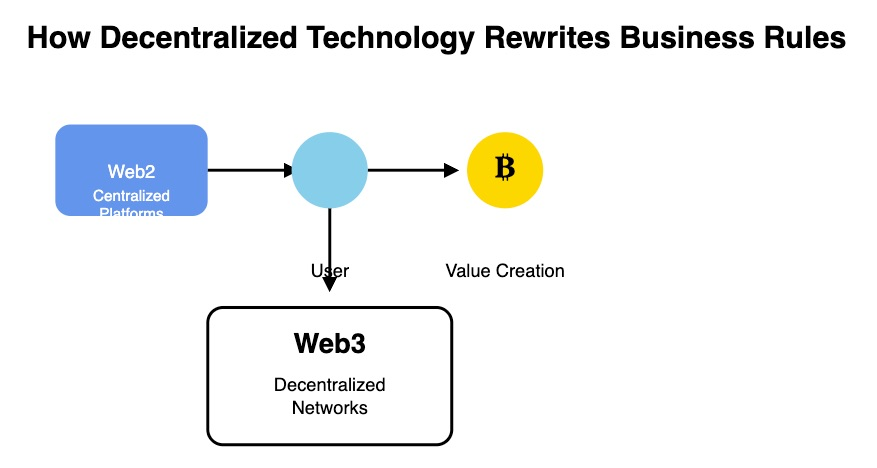
\includegraphics[keepaspectratio]{_resources/assets/images/ch2-overview.jpg}}

\section{数据主权革命}\label{ux6570ux636eux4e3bux6743ux9769ux547d}

Web3技术引入了数据主权的可能性,从根本上改变了平台和用户之间的权力平衡。在当前系统中,每次点击、购买、搜索和互动都会产生流向平台所有者的数据,他们使用这些信息来优化自己的收入生成。用户无法了解他们的数据如何被收集、处理或货币化,也没有收到他们的活动创造的价值的补偿。

去中心化身份系统使个人能够跨多个平台和应用程序拥有和控制他们的数字身份。用户不再为每项服务创建单独账户并向每个平台交出个人信息,而是可以维护他们完全控制的便携式身份。这种转变对数字商业如何运作具有深远影响,因为它消除了平台通过数据锁定效应困住用户的能力。

当用户拥有他们的数据时,他们可以选择与不同服务分享哪些信息以及在什么条件下分享。他们可以授予可以随时撤销的临时访问权限。最重要的是,他们可以就分享有价值的数据或参与数据生成活动进行补偿谈判。这为数据交换创造了市场机制,而不是当前的无补偿提取系统。

这种影响延伸到商业环境中的客户关系。通过Web3系统与客户互动的商家可以在没有中介平台控制访问的情况下发展直接关系。客户数据仍然属于客户,他们可以选择直接与他们信任的商家分享购买历史、偏好和其他有价值的信息。这使得企业和客户之间建立更真实的关系成为可能,同时无需对这些互动征收平台税。

去中心化存储系统确保用户数据不会被平台所有者丢失、损坏或操纵。存储在分布式网络上的信息对用户保持可访问,无论任何特定平台或服务提供商发生什么。这创造了真正的数据可移植性,使用户能够在服务之间移动,同时保持其数字历史和关系。

数据主权革命还通过用户参与实现新形式的价值创造。当用户拥有他们的数据和互动时,他们可以选择直接将这些资产货币化,而不是允许平台捕获所有价值。这可能涉及向研究人员出售数据、参与产生直接收入的内容创作,或为创造代币化奖励的网络效应做出贡献。

\section{从消费者到利益相关者}\label{ux4eceux6d88ux8d39ux8005ux5230ux5229ux76caux76f8ux5173ux8005}

传统平台关系将用户定位为购买产品或服务以换取金钱的消费者,或作为提供材料以换取平台中介收入分享的内容创作者。Web3系统实现了基本角色转换,用户成为在他们帮助创建和维护的平台和网络中拥有所有权利益的利益相关者。

这种转换通过基于代币的所有权系统发生,该系统根据网络参与者对网络价值的贡献,在他们之间分配经济权利。参与者不再为捕获用户活动大部分价值的平台工作,而是可以在他们帮助建设和维护的网络中获得所有权股份。这些所有权股份通常采用治理代币的形式,提供网络决策的投票权,以及使持有者有权获得网络收入份额的经济代币。

利益相关者模式以平台系统无法实现的方式在平台和参与者之间调整激励。当用户拥有他们参与的网络的一部分时,他们直接从网络增长和成功中受益。这为用户贡献高质量内容、提供有用反馈、招募新参与者以及以其他方式支持网络发展创造了强大的激励。结果通常是比中心化平台通过纯粹提取关系能够实现的更快增长和更高质量的结果。

与利益相关者地位相关的治理权利使得真正的民主参与平台发展和政策决定成为可能。利益相关者不再接受平台所有者决定实施的任何变化,而是可以提出修改、对重要决定进行投票,并集体指导网络演进。这创造了保持响应参与者需求而不是仅为所有者利益优化的系统。

利益相关者参与的经济影响随着成功网络增长而随时间复合。帮助建立和发展网络的早期参与者可以看到其所有权股份的实质性升值,因为网络实现规模和采用。这为长期承诺和高质量参与创造了激励,而不是许多平台关系特征的短期提取。

此外,利益相关者模式使风险分担和网络发展中的协作投资成为可能。当参与者拥有所有权股份时,他们愿意在网络改进中投资时间、金钱和努力,因为他们将分享这些投资的收益。与只有平台所有者从网络改进中受益的系统相比,这可以加速创新和发展。

\section{智能合约商业}\label{ux667aux80fdux5408ux7ea6ux5546ux4e1a}

智能合约代表Web3技术中最重要的创新之一,使协议的自动执行成为可能,而无需可信的中介。在商业环境中,智能合约可以自动化支付处理、执行服务协议、分配收入份额,并以数学精度和完全透明度管理复杂的多方交易。

通过智能合约自动化消除中介降低了交易成本,同时提高了执行的可靠性和速度。传统商业交易通常需要银行、支付处理器、托管服务和其他中介来确保所有方履行其义务。每个中介都为交易过程增加成本、复杂性和潜在故障点。智能合约可以用自动代码替换许多这些中介,当满足指定条件时,自动代码执行预定义的逻辑。

考虑涉及商家、客户、支付处理器和运输公司的典型电子商务交易。传统系统需要多个中介来协调这些互动,每个都收取费用并引入延迟。智能合约系统可以在货物交付时自动处理付款,向商家和运输公司分配适当的部分,处理税收计算,并在出现问题时触发客户服务流程。整个交易根据预定义的规则执行,无需人工干预或中介协调。

智能合约还使通过传统系统管理起来不切实际的更复杂商业安排成为可能。多方之间的收入分享协议可以自动化,以确保根据复杂公式准确及时地分配资金。订阅服务可以根据使用模式或市场条件自动调整定价。当触发事件发生时,保险索赔可以自动处理。这些能力使新的商业模式成为可能,这些模式以前太复杂或太昂贵而无法实施。

智能合约系统的透明度通过使所有交易逻辑可见和可验证,在商业伙伴之间建立信任。参与者可以检查管理其互动的代码,确保自动化系统将按预期运行。这种透明度减少了争议,并使可能不会相互信任履行复杂协议的各方之间的合作成为可能。

智能合约还使可编程货币成为可能,可以自动执行支出规则、储蓄目标和投资策略。个人不再依赖个人纪律或第三方金融服务,而是可以创建自动化系统,根据预定规则分配收入,投资多元化投资组合,并执行复杂的金融策略,而无需持续的手动管理。

\section{中介的消亡}\label{ux4e2dux4ecbux7684ux6d88ux4ea1}

Web3技术使直接的点对点交易成为可能,消除了许多传统中介角色,同时通过网络参与创造新形式的价值创造。参与者不再向中介支付费用来促进交易,而是可以直接互动,同时为服务其集体利益的共享基础设施做出贡献。

去中心化金融协议展示了中介消除在实践中如何运作。传统银行要求客户将钱存入金融机构,然后将这些资金借给借款人,同时捕获利率差价。DeFi协议使存款人能够通过自动化系统直接借给借款人,通常获得更高的回报,而借款人支付更低的利率。中介利润被消除,储蓄在贷款人和借款人之间分享。

类似的动态适用于许多其他商业部门。内容创作者可以通过去中心化平台直接向观众分发他们的作品,保留更大部分的收入,否则这些收入将流向平台中介。自由职业者可以通过收取与传统自由职业平台相比微不足道费用的点对点网络与客户联系。商家可以通过收取比中心化平台更少佣金的去中心化市场直接向消费者销售。

中介的消除并不意味着消除中介传统提供的有价值服务。相反,这些服务在网络参与者之间分布或通过智能合约自动化。质量保证、争议解决、支付处理和其他中介功能继续存在,但通过去中心化机制而不是中心化中介提供。

这种转换为个人创造了通过在去中心化网络内提供特定服务而不是为中介公司工作来赚取收入的机会。网络参与者可以通过内容审核、争议解决、质量验证、客户服务和许多其他以前由平台员工执行的功能获得奖励。这为个人创造了更灵活且通常更有利可图的机会,同时降低了与中心化中介组织相关的开销成本。

传统中介的消亡还使生产者和消费者之间更直接的关系成为可能,导致更好的价格发现和更高效的市场。当移除多层中介时,生产者和消费者都可以通过其互动捕获创造价值的更大部分。这通常导致消费者价格更低,生产者收入更高,差异代表消除中介提取。

\section{对商业策略的影响}\label{ux5bf9ux5546ux4e1aux7b56ux7565ux7684ux5f71ux54cd}

向Web3商业的过渡要求企业在客户获取、关系管理和价值创造方面采取根本性改变。理解并适应这些变化的公司将发现显著的竞争优势,而那些坚持依赖平台策略的公司可能发现自己越来越处于劣势。

Web3环境中的客户获取专注于提供真正价值和建立信任,而不是通过广告平台购买注意力。由于Web3用户拥有他们的数据和身份,他们可以更容易地评估和比较不同选项。企业必须基于提供的实际价值而不是营销复杂性或广告支出能力进行竞争。

关系管理从平台中介的互动转向与拥有其数据和身份的客户的直接参与。这使得更深入、更真实的关系成为可能,但要求企业提供持续价值,而不是依赖平台锁定效应来维持客户忠诚度。在为客户创造真正价值方面表现出色的公司将蓬勃发展,而那些依赖信息不对称或转换成本的公司将面临困难。

在Web3环境中,价值创造机会显著扩大,因为企业可以参与网络效应和代币经济,而不是简单地从交易中提取利润。公司可以创建并参与随着吸引更多参与者而增长价值的去中心化网络。这可以提供通过传统商业模式无法获得的指数增长机会。

Web3转型既代表技术转变,也代表向更公平、更高效的数字商业形式的哲学演进。正如我们将在第三章中探讨的,这些原则的实际实施需要平台设计、代币经济学和社区治理的系统方法。链上商业的六大支柱提供了一个框架,用于理解这些抽象概念如何转化为能够大规模运营同时保持去中心化和参与者所有权好处的具体商业系统。

\chapter{第三章:链上商业的六大支柱}\label{sec-six-pillars}

链上商业系统的成功不是偶然的,而是建立在六个相互支撑的核心支柱之上。这些支柱共同构成了一个自我维持、自我发展的商业生态系统。

\section{支柱一:公平利润分享机制}\label{ux652fux67f1ux4e00ux516cux5e73ux5229ux6da6ux5206ux4eabux673aux5236}

\subsection{传统模式的问题}\label{ux4f20ux7edfux6a21ux5f0fux7684ux95eeux9898}

在传统商业模式中,利润分配往往是不透明和不公平的: - 平台获得大部分价值
- 创造者获得微薄收益 - 用户无法分享价值增长

\subsection{链上商业的解决方案}\label{ux94feux4e0aux5546ux4e1aux7684ux89e3ux51b3ux65b9ux6848}

通过智能合约实现的自动化利润分享:

\begin{Shaded}
\begin{Highlighting}[]
\NormalTok{contract ProfitSharing \{}
\NormalTok{    struct Participant \{}
\NormalTok{        uint256 contribution;}
\NormalTok{        uint256 rewards;}
\NormalTok{        uint256 lastClaim;}
\NormalTok{    \}}
    
\NormalTok{    mapping(address =\textgreater{} Participant) public participants;}
\NormalTok{    uint256 public totalRewards;}
    
\NormalTok{    function distributeRewards() external \{}
\NormalTok{        // 基于贡献自动分配奖励}
\NormalTok{        for (address participant : participants) \{}
\NormalTok{            uint256 share = calculateShare(participant);}
\NormalTok{            participants[participant].rewards += share;}
\NormalTok{        \}}
\NormalTok{    \}}
\NormalTok{\}}
\end{Highlighting}
\end{Shaded}

\subsection{实施特点}\label{ux5b9eux65bdux7279ux70b9}

\begin{enumerate}
\def\labelenumi{\arabic{enumi}.}
\tightlist
\item
  \textbf{透明性}:所有分配规则在链上公开
\item
  \textbf{自动化}:无需人工干预,智能合约自动执行
\item
  \textbf{实时性}:奖励实时计算和分配
\item
  \textbf{公平性}:基于实际贡献进行分配
\end{enumerate}

\section{支柱二:稳定代币价值支撑模型}\label{ux652fux67f1ux4e8cux7a33ux5b9aux4ee3ux5e01ux4ef7ux503cux652fux6491ux6a21ux578b}

\subsection{价值稳定的重要性}\label{ux4ef7ux503cux7a33ux5b9aux7684ux91cdux8981ux6027}

代币价值的稳定性直接影响生态系统的健康发展: - 过度波动影响用户信心 -
投机性质削弱实用价值 - 价格操控损害公平性

\subsection{多重稳定机制}\label{ux591aux91cdux7a33ux5b9aux673aux5236}

\begin{enumerate}
\def\labelenumi{\arabic{enumi}.}
\item
  \textbf{储备金支撑}

  \begin{itemize}
  \tightlist
  \item
    建立多元化资产储备
  \item
    设置自动调节机制
  \item
    透明的储备证明系统
  \end{itemize}
\item
  \textbf{实际价值锚定}

  \begin{itemize}
  \tightlist
  \item
    与真实商业交易绑定
  \item
    基于网络使用量调节供应
  \item
    避免纯投机驱动
  \end{itemize}
\item
  \textbf{算法稳定机制}

\begin{Shaded}
\begin{Highlighting}[]
\NormalTok{contract TokenStabilizer \{}
\NormalTok{    uint256 public targetPrice;}
\NormalTok{    uint256 public currentSupply;}

\NormalTok{    function adjustSupply() external \{}
\NormalTok{        uint256 currentPrice = getCurrentPrice();}
\NormalTok{        if (currentPrice \textgreater{} targetPrice) \{}
\NormalTok{            // 增加供应量}
\NormalTok{            mint(calculateMintAmount());}
\NormalTok{        \} else if (currentPrice \textless{} targetPrice) \{}
\NormalTok{            // 减少供应量}
\NormalTok{            burn(calculateBurnAmount());}
\NormalTok{        \}}
\NormalTok{    \}}
\NormalTok{\}}
\end{Highlighting}
\end{Shaded}
\end{enumerate}

\section{支柱三:可扩展的商家成长阶梯}\label{ux652fux67f1ux4e09ux53efux6269ux5c55ux7684ux5546ux5bb6ux6210ux957fux9636ux68af}

\subsection{成长路径设计}\label{ux6210ux957fux8defux5f84ux8bbeux8ba1}

链上商业为不同规模的参与者提供清晰的成长路径:

\begin{enumerate}
\def\labelenumi{\arabic{enumi}.}
\tightlist
\item
  \textbf{个人创作者阶段}

  \begin{itemize}
  \tightlist
  \item
    内容创作和分享
  \item
    基础代币奖励
  \item
    社区建设起步
  \end{itemize}
\item
  \textbf{小型商家阶段}

  \begin{itemize}
  \tightlist
  \item
    产品或服务销售
  \item
    客户关系管理
  \item
    品牌建设发展
  \end{itemize}
\item
  \textbf{区域合作伙伴阶段}

  \begin{itemize}
  \tightlist
  \item
    多商家协调
  \item
    区域网络管理
  \item
    规模效应获得
  \end{itemize}
\item
  \textbf{生态节点阶段}

  \begin{itemize}
  \tightlist
  \item
    技术基础设施运营
  \item
    治理参与权重增加
  \item
    网络收益最大化
  \end{itemize}
\end{enumerate}

\subsection{激励机制设计}\label{ux6fc0ux52b1ux673aux5236ux8bbeux8ba1}

每个阶段都有相应的激励机制:

\begin{Shaded}
\begin{Highlighting}[]
\NormalTok{contract GrowthIncentives \{}
\NormalTok{    enum Level \{ Creator, Merchant, Partner, Node \}}
    
\NormalTok{    struct Participant \{}
\NormalTok{        Level currentLevel;}
\NormalTok{        uint256 contributionScore;}
\NormalTok{        uint256 rewardMultiplier;}
\NormalTok{    \}}
    
\NormalTok{    function levelUp(address participant) external \{}
\NormalTok{        Participant storage p = participants[participant];}
\NormalTok{        if (p.contributionScore \textgreater{}= getThreshold(p.currentLevel)) \{}
\NormalTok{            p.currentLevel = Level(uint(p.currentLevel) + 1);}
\NormalTok{            p.rewardMultiplier = getMultiplier(p.currentLevel);}
\NormalTok{        \}}
\NormalTok{    \}}
\NormalTok{\}}
\end{Highlighting}
\end{Shaded}

\section{支柱四:高信任社区网络}\label{ux652fux67f1ux56dbux9ad8ux4fe1ux4efbux793eux533aux7f51ux7edc}

\subsection{信任机制构建}\label{ux4fe1ux4efbux673aux5236ux6784ux5efa}

\begin{enumerate}
\def\labelenumi{\arabic{enumi}.}
\tightlist
\item
  \textbf{声誉系统}

  \begin{itemize}
  \tightlist
  \item
    基于历史行为的信誉评分
  \item
    多维度评价体系
  \item
    去中心化评价机制
  \end{itemize}
\item
  \textbf{质押保证}

  \begin{itemize}
  \tightlist
  \item
    参与者质押代币作为保证金
  \item
    不当行为导致质押损失
  \item
    良好行为获得奖励
  \end{itemize}
\item
  \textbf{社区治理}

  \begin{itemize}
  \tightlist
  \item
    去中心化自治组织(DAO)
  \item
    提案和投票机制
  \item
    透明的决策过程
  \end{itemize}
\end{enumerate}

\subsection{网络结构优化}\label{ux7f51ux7edcux7ed3ux6784ux4f18ux5316}

不同于传统的金字塔结构,链上商业采用网状结构: - 每个节点都是价值创造者
- 横向合作优于纵向控制 - 网络效应惠及所有参与者

\section{支柱五:真正的''共享''利润分配}\label{ux652fux67f1ux4e94ux771fux6b63ux7684ux5171ux4eabux5229ux6da6ux5206ux914d}

\subsection{共享经济的重新定义}\label{ux5171ux4eabux7ecfux6d4eux7684ux91cdux65b0ux5b9aux4e49}

传统''共享经济''实际上是''平台经济'': - 资产所有者获得微薄收入 -
平台获得大部分价值 - 用户承担大部分风险

\subsection{链上商业的共享模式}\label{ux94feux4e0aux5546ux4e1aux7684ux5171ux4eabux6a21ux5f0f}

\begin{enumerate}
\def\labelenumi{\arabic{enumi}.}
\tightlist
\item
  \textbf{所有权共享}

  \begin{itemize}
  \tightlist
  \item
    参与者共同拥有网络
  \item
    代币代表网络股权
  \item
    价值增长共同受益
  \end{itemize}
\item
  \textbf{收益共享}

  \begin{itemize}
  \tightlist
  \item
    网络收入按贡献分配
  \item
    无中心化机构抽取
  \item
    透明化分配机制
  \end{itemize}
\item
  \textbf{治理共享}

  \begin{itemize}
  \tightlist
  \item
    重大决策集体投票
  \item
    每个代币持有者都有发言权
  \item
    去中心化治理结构
  \end{itemize}
\end{enumerate}

\section{支柱六:高频次必需场景}\label{ux652fux67f1ux516dux9ad8ux9891ux6b21ux5fc5ux9700ux573aux666f}

\subsection{实用性优先}\label{ux5b9eux7528ux6027ux4f18ux5148}

链上商业必须解决真实世界的问题:

\begin{enumerate}
\def\labelenumi{\arabic{enumi}.}
\tightlist
\item
  \textbf{日常消费场景}

  \begin{itemize}
  \tightlist
  \item
    食品、服装、日用品
  \item
    服务预订和支付
  \item
    本地商户网络
  \end{itemize}
\item
  \textbf{商业服务场景}

  \begin{itemize}
  \tightlist
  \item
    供应链管理
  \item
    物流协调
  \item
    资金流转
  \end{itemize}
\item
  \textbf{数字服务场景}

  \begin{itemize}
  \tightlist
  \item
    内容消费
  \item
    教育培训
  \item
    娱乐互动
  \end{itemize}
\end{enumerate}

\subsection{技术实现}\label{ux6280ux672fux5b9eux73b0}

高频场景需要高性能的技术支撑:

\begin{Shaded}
\begin{Highlighting}[]
\NormalTok{contract HighFrequencyCommerce \{}
\NormalTok{    mapping(bytes32 =\textgreater{} Transaction) public transactions;}
    
\NormalTok{    struct Transaction \{}
\NormalTok{        address buyer;}
\NormalTok{        address seller;}
\NormalTok{        uint256 amount;}
\NormalTok{        uint256 timestamp;}
\NormalTok{        bool completed;}
\NormalTok{    \}}
    
\NormalTok{    function quickPayment(}
\NormalTok{        address seller,}
\NormalTok{        uint256 amount,}
\NormalTok{        bytes calldata data}
\NormalTok{    ) external \{}
\NormalTok{        // 优化的快速支付流程}
\NormalTok{        bytes32 txId = keccak256(abi.encode(}
\NormalTok{            msg.sender, seller, amount, block.timestamp}
\NormalTok{        ));}
        
\NormalTok{        transactions[txId] = Transaction(\{}
\NormalTok{            buyer: msg.sender,}
\NormalTok{            seller: seller,}
\NormalTok{            amount: amount,}
\NormalTok{            timestamp: block.timestamp,}
\NormalTok{            completed: true}
\NormalTok{        \});}
        
\NormalTok{        // 即时执行奖励分配}
\NormalTok{        distributeRewards(txId);}
\NormalTok{    \}}
\NormalTok{\}}
\end{Highlighting}
\end{Shaded}

\section{六大支柱的协同效应}\label{ux516dux5927ux652fux67f1ux7684ux534fux540cux6548ux5e94}

这六大支柱不是独立存在的,而是相互增强的:

\begin{enumerate}
\def\labelenumi{\arabic{enumi}.}
\tightlist
\item
  \textbf{公平分享} + \textbf{稳定价值} = 可预期的收益
\item
  \textbf{成长阶梯} + \textbf{信任网络} = 可持续发展
\item
  \textbf{共享治理} + \textbf{实用场景} = 真实价值创造
\end{enumerate}

\subsection{系统稳定性}\label{ux7cfbux7edfux7a33ux5b9aux6027}

通过六大支柱的相互支撑,链上商业系统具备了: -
\textbf{抗冲击能力}:单一支柱问题不会导致系统崩溃 -
\textbf{自我修复能力}:系统能够自动调节和优化 -
\textbf{持续进化能力}:随着网络发展不断完善

\section{实施路线图}\label{ux5b9eux65bdux8defux7ebfux56fe}

\subsection{短期目标(0-6个月)}\label{ux77edux671fux76eeux68070-6ux4e2aux6708}

\begin{itemize}
\tightlist
\item
  部署核心智能合约
\item
  建立基础激励机制
\item
  吸引早期参与者
\end{itemize}

\subsection{中期目标(6-18个月)}\label{ux4e2dux671fux76eeux68076-18ux4e2aux6708}

\begin{itemize}
\tightlist
\item
  完善治理结构
\item
  扩展应用场景
\item
  优化用户体验
\end{itemize}

\subsection{长期目标(18个月以上)}\label{ux957fux671fux76eeux680718ux4e2aux6708ux4ee5ux4e0a}

\begin{itemize}
\tightlist
\item
  实现生态自治
\item
  扩展全球网络
\item
  持续价值创新
\end{itemize}

\section{总结}\label{ux603bux7ed3}

六大支柱构成了链上商业的核心框架。它们不仅解决了传统商业模式的痛点,更重要的是创建了一个可持续发展的价值创造生态系统。

在下一章中,我们将深入探讨''花得越多,赚得越多''的系统机制,以及如何通过技术手段实现这一看似矛盾的商业逻辑。

\part{第二部分:轉型機制}

\chapter{第四章:``花得越多,赚得越多''运营系统}\label{sec-spend-earn-system}

消费如何在新经济中成为投资

花钱实际上可以增加财富而不是减少财富这一概念,代表了链上商业系统最反直觉的方面之一。传统经济思维将消费和投资视为对立活动:用于商品和服务的钱不再可用于财富建设投资。链上商业通过创建消费活动同时为参与者生成投资回报的机制,从根本上重构了这种关系。

这种转换通过复杂的代币分配系统发生,该系统将消费者支出的一部分转换为可交易的数字资产,同时保持表征正常商业交易的基本价值交换。客户收到他们购买的商品和服务,同时还收到代表在促成其购买的商业网络中的所有权股份的代币。结果是一个系统,其中增加的参与和支出产生增加的财富积累,而不是耗尽财政资源。

理解这个系统如何运作需要检查传统消费支出转换为投资资产的具体机制,确保可持续回报的数学基础,以及使这样的系统能够创造真正价值而不是简单地在参与者之间重新分配现有财富的经济原则。

\section{交易到资产转换}\label{ux4ea4ux6613ux5230ux8d44ux4ea7ux8f6cux6362}

花得越多赚得越多系统的基础机制在于将交易金额自动转换为随时间升值的代币资产。当客户通过链上商业平台进行购买时,商家的利润分享承诺立即转换为Apollo
Coin(AC)代币,根据预定分配公式分配给客户和其他网络参与者。

这种转换过程通过智能合约运作,智能合约自动执行复杂的计算和分配,而不需要人工干预或对第三方管理员的信任。商家设定利润分享百分比,代表他们愿意分配给网络代币分配的总销售额部分。这个百分比通常从交易价值的3\%到99\%不等,代表商家为了换取参与链上商业网络产生的营销利益和客户忠诚度而放弃的真实经济价值。

考虑这种转换在实践中如何运作的具体例子。客户在参与链上商业并承诺30\%利润分享的餐厅购买50美元的餐食。客户支付50美元并收到他们的餐食,完全如同任何传统交易。然而,智能合约系统还自动将15美元(50美元的30\%)根据当前市场汇率转换为AC代币,并根据网络的分配公式分配这些代币。

使用第三章讨论的分配模型,转换金额的60\%将作为奖励流向客户,15\%作为参与激励流向商家,4\%流向推荐伙伴,3\%流向区域协调员,其余18\%在各种网络基础设施参与者之间分配。这意味着客户将收到价值9美元的AC代币,而商家收到价值2.25美元的代币,尽管已经向转换池贡献了15美元的利润率。

交易到资产转换为客户创造即时价值,同时建立通过增加的客户忠诚度和重复业务使商家受益的长期关系。客户产生返回参与商家的财务激励,因为他们的支出通过代币升值产生持续的投资回报。商家从降低的客户获取成本和增加的交易频率中受益,通常超过分配给代币分配的利润率的补偿。

转换机制还创造了网络效应,随着系统增长使所有参与者受益。每笔交易都加强了AC代币的储备支撑,同时展示了对网络服务的真实经济需求。储备加强和需求验证的结合支持代币价值升值,使整个网络中的所有代币持有者受益。

此外,交易到资产转换的自动性质消除了通常阻止消费者参与传统投资计划的复杂性和障碍。客户不需要理解代币机制、管理数字钱包或做出明确的投资决策。转换作为正常购物活动的一部分无缝发生,使投资参与对可能永远不会参与传统加密货币或投资系统的个人可及。

\section{AC代币经济}\label{acux4ee3ux5e01ux7ecfux6d4e}

Apollo
Coin代币经济提供了使可持续花得越多赚得越多运营成为可能的数学基础。与主要从交易活动和市场情绪获得价值的投机性加密货币不同,AC代币由通过实际商业交易产生的真实经济储备支撑。这种支撑创造了内在价值,支持基于基本经济活动而不是投机泡沫的长期价格稳定和升值。

储备支撑系统通过去中心化智能合约运作,自动将商家利润分享贡献的一部分存入储备池。这些储备以稳定的加密货币如USDC(美元币)持有,与传统货币保持可靠的价值关系。储备池为AC代币价值提供数学支持,同时使代币持有者能够在特定条件下将代币兑换为基础储备资产。

流通的AC代币和储备支撑之间的关系创造了自然的价格稳定机制。当AC代币交易低于其储备支撑的内在价值时,出现购买被低估代币并可能将其兑换为更高价值储备资产的套利机会。相反,当代币交易高于内在价值时,通过新商家交易的额外代币创建增加供应,直到价格在数学支持水平附近稳定。

代币经济还包含鼓励流通而不是囤积的速度激励。在网络内用于购买的AC代币比作为静态投资持有时产生额外价值。积极与参与商家消费AC代币的网络参与者通常收到奖金分配、推荐奖励或其他激励,与被动持有者相比增加他们的总代币积累。

AC代币分配基础的数学模型确保网络增长创造正和结果而不是零和重新分配。随着更多商家加入网络并向储备池贡献利润分享,所有未偿代币的总支撑增加。同时,增加的商家参与为代币利用创造更多机会,通过基本供需动态产生支持价格升值的需求。

地理扩张战略通过创建支持代币实用性和需求的多个区域市场进一步加强代币经济。当特定地理区域内的足够商家参与网络时,客户可以将AC代币用于他们的许多日常购买,创造超越投机交易价值的实用性。这种基于实用性的需求为代币价值提供可持续支持,独立于加密货币市场波动。

储备支撑和代币分配的透明度创造了在系统长期可持续性中建立参与者信心的问责制。与依赖机构承诺或复杂金融工程的传统投资计划不同,AC代币持有者可以通过基于区块链的审计系统验证其代币持有和基础储备资产之间的数学关系。

\section{闭环价值系统}\label{ux95edux73afux4ef7ux503cux7cfbux7edf}

花得越多赚得越多系统最复杂的方面在于创建闭环价值系统,这些系统放大参与者的利益,同时减少对外部经济条件的依赖。这些系统通过创建多个相互关联的价值流来实现可持续性,这些价值流通过网络效应和参与者行为优化相互加强。

主要循环通过客户支出、代币积累和网络内再投资运作。通过购买收到AC代币的客户被激励与其他网络商家消费这些代币,既为了利用其代币价值,又为了通过持续的网络参与产生额外的代币奖励。这创造了一个流通模式,其中代币在客户和商家之间流动,同时在每个交易点产生增量价值。

通过推荐和社区建设活动出现次级循环,这些活动扩展网络参与并增加总交易量。成功为网络招募新商家或客户的参与者从其推荐产生的增加活动中获得持续补偿。这为网络传播和增长创造激励,通过增加代币实用性和升值而不是简单地在更多参与者之间稀释现有价值来使现有参与者受益。

商家生态系统通过协作和交叉推荐活动创造额外的价值循环。参与的商家经常发展互补关系,他们为其专业之外的服务相互推荐客户。餐厅可能与附近的水疗中心、零售店或娱乐场所合作,创建全面的本地网络,增加客户便利性,同时为参与企业产生推荐收入。

区域协调机制使本地商家网络能够汇集资源用于营销活动、客户获取计划和基础设施开发,使所有网络参与者受益。这些协作投资产生根据其贡献水平和网络活动在参与商家之间分配的回报,为集体而不是纯粹个人优化创造激励。

闭环系统还包含基于参与者行为和结果优化网络性能的反馈机制。分析系统跟踪客户满意度、商家盈利能力、代币流通模式和网络增长指标,以识别优化机会并调整系统参数以改善性能。这种持续改进过程确保网络演进以更好地服务参与者需求,同时保持数学可持续性。

质量保证循环通过监控商家绩效和客户满意度水平来维护网络完整性。始终提供积极客户体验的商家获得增强的利益和促销支持,而那些产生投诉或负面反馈的商家可能面临减少的参与利益或从网络中移除。这为保护网络声誉和客户保留的服务质量创造激励。

多个价值循环的整合创造了抵御外部经济破坏的韧性。当传统经济条件恶化时,闭环网络可以通过内部流通和交换活动继续为参与者创造价值。这种韧性在经济不确定性期间变得特别有价值,当传统投资和就业机会可能变得不太可靠时。

\section{风险缓解和系统保障}\label{ux98ceux9669ux7f13ux89e3ux548cux7cfbux7edfux4fddux969c}

花得越多赚得越多模式包含全面的风险缓解策略,将其与赌博、投机或不可持续的金融计划区别开来。这些保障保护参与者投资,同时通过保守的数学模型和透明的操作程序确保系统可持续性。

储备支撑要求确保代币价值由真实经济资产而不是投机市场情绪支撑。相对于未偿代币的储备支撑百分比通过算法控制维持,防止相对于可用储备资金的代币过度发行。这为代币价值创造数学底限,保护参与者免受表征纯粹投机投资的全部损失情况。

商家审查程序在企业能够参与利润分享计划之前验证其合法性和可持续性。新商家必须展示稳定的业务运营、适当的许可和注册,以及足够的交易量来支持其提议的利润分享承诺。这种筛选过程减少了可能损害网络完整性的欺诈或不可持续商家参与的风险。

交易限制防止个人参与者相对于其财务能力冒过度风险。通过支出活动获取代币的每日、每周和每月限制确保参与者不能相对于其整体财务状况无意中过度投资网络代币。这些限制可以根据参与者收入验证和对系统运营的展示理解进行调整。

地理多元化将网络风险分散到多个区域市场和经济条件中。链上商业网络不是将所有活动集中在单一地点或行业,而是故意在地理区域和商业部门中培养商家多样性。这种多元化减少了地方经济破坏对整体网络稳定性和参与者回报的影响。

治理机制使参与者能够输入系统修改和风险管理政策。代币持有者可以提议并投票表决储备要求、分配公式、商家资格标准和影响网络运营和参与者安全的其他系统参数的变化。这种民主治理确保风险管理政策反映参与者偏好和不断变化的市场条件。

法规合规程序确保网络运营符合适用的金融法规和消费者保护法。管理证券、支付处理、消费者保护和税收的法律框架被仔细分析并纳入系统设计,以防止可能威胁网络运营或参与者利益的法规冲突。

退出机制使参与者能够在各种情况下收回其投资。代币赎回选择、商家退出程序和客户退款政策为参与者在其情况或偏好发生变化时退出网络提供多种途径。这些退出选择通过有序的离开程序减少参与者风险,同时维护网络完整性。

\section{投资回报分析}\label{ux6295ux8d44ux56deux62a5ux5206ux6790}

花得越多赚得越多系统的数学基础使得能够在各种情景和市场条件下对参与者回报进行定量分析。这些计算展示了普通支出活动如何产生类似投资的回报,同时保持正常商业交易的实用效用。

即时回报组件来自代币分配百分比,从客户的购买中向他们提供即时价值。从承诺30\%利润分享的商家购买100美元商品的客户将立即收到价值18美元的AC代币(30美元转换金额的60\%)。这代表支出的即时18\%回报,与高收益投资回报相当,但通过正常消费活动实现。

升值组件取决于网络增长和代币价值随时间增加。成功链上商业实施的历史分析展示了年度代币升值率从20\%到300\%不等,取决于网络采用率和区域经济条件。基于可持续增长模型的保守预测表明,在有利但现实的条件下,代币价值可能每年升值50\%到100\%。

复合增长组件来自在网络内再投资代币以产生额外代币积累。使用其AC代币进行后续购买的客户继续赚取额外代币,同时从其现有代币持有的任何升值中受益。这种复合效应可以随时间显著放大总回报,特别是对于保持高水平网络参与的参与者。

区域网络效应通过跨商家利用和推荐计划创造额外的回报机会。成熟区域网络中的参与者在结合即时代币分配、升值收益、推荐收入和网络参与奖励时,经常报告超过其支出活动200\%的总年回报。这些回报反映了当足够的商家和客户参与本地化链上商业生态系统时出现的网络效应。

风险调整回报计算考虑了潜在的代币价值波动和网络采用不确定性。即使在假设适度网络增长和有限代币升值的保守情景下,参与者通常实现超过传统储蓄账户、货币市场基金和许多传统投资选择的正回报。即时代币分配和适度升值的结合通常产生从纯财务角度证明参与合理的回报。

增加购买力的实际好处通过改善网络商家社区内商品和服务的获取进一步增强有效回报。参与者经常发现新业务,从网络商家获得优惠待遇,并获得提供超越纯财务回报价值的独家优惠和服务。这些定性好处补充定量回报,创造证明网络参与合理的综合价值主张。

长期财富建设潜力来自在多年期间持续参与不断增长的链上商业网络。在扩展网络中保持一致参与和再投资的参与者经常积累随着网络实现区域或国家规模而显著升值的大量代币持有。这种财富建设潜力将日常支出活动转化为可以产生实质性长期财务好处的系统投资计划。

花得越多赚得越多运营系统代表了消费者经济学的基本创新,将个人支出决策与投资回报结合,同时支持真正的业务发展和社区繁荣。正如我们将在第五章中探讨的,这个系统与传统的多级营销、电子商务和特许经营模式截然不同,这些模式经常在个人和集体利益之间创造冲突。链上商业的数学基础和系统保障创造可持续的价值生成,使所有参与者受益,同时服务于本地和区域市场的真实经济需求。

\chapter{第五章:超越传销、电商和特许经营}\label{sec-beyond-traditional}

与传统商业模式的根本差异

链上商业系统经常被误解为多级营销、电子商务平台或特许经营运营的变体,因为它们与这些传统商业模式共享某些表面特征。所有这些都涉及参与者网络、多方之间的收入分享,以及通过参与者招募和保留实现增长。然而,链上商业的基本结构、激励系统和价值创造机制与这些传统方法截然不同,以解决限制其可持续性和公平性的系统性问题的方式。

理解这些差异需要检查的不仅是每种模式的操作机制,还有决定其长期可行性和对参与者影响的基础经济原理和激励结构。虽然传统模式经常在个人成功和集体可持续性之间创造冲突,但链上商业通过精心设计的代币经济学和治理机制调整个人和集体利益。

这种区别很重要,因为许多有前途的商业创新由于建立在从传统模式借用的有缺陷的基础假设上而失败。链上商业代表了一种真正新的商业组织方法,超越现有框架的限制,同时保留其有益元素。

\section{传销陷阱:多级营销的结构缺陷}\label{ux4f20ux9500ux9677ux9631ux591aux7ea7ux8425ux9500ux7684ux7ed3ux6784ux7f3aux9677}

多级营销系统创造分布式机会的外观,同时实际上以后期加入者为代价,在早期参与者中集中财富和权力。MLM系统的数学结构确保绝大多数参与者将亏损,而一小部分实现实质性回报,创造不可避免地导致系统崩溃的不可持续动态。

MLM系统的根本缺陷在于它们依赖指数招募增长来为现有参与者产生收入。每个参与者必须招募多个新参与者,每个新参与者必须招募额外的参与者来维持收入水平。这创造了金字塔结构,其中早期参与者从越来越多的后期参与者的努力中受益,而没有提供相称的回报价值。

考虑典型MLM结构的数学,其中每个参与者需要招募五个新参与者才能实现有意义的收入。在五个层级的招募后,系统需要超过三千名参与者在底层支持大约六百名更高层级的参与者。在十个层级后,底层需要数百万参与者,迅速超过大多数市场的可用人口。这种数学不可能性保证大多数参与者将失败实现有意义的回报,无论他们的努力或技能如何。

MLM系统还创造优先考虑招募而不是实际价值创造的不当激励。参与者通过招募新分销商比通过向最终客户销售产品赚更多钱,导致专注于销售演示和招募活动而不是客户服务和产品改进。这种不匹配经常导致糟糕的客户体验和无法在正常市场条件下有效竞争的低质量产品。

MLM系统中常见的库存装载要求迫使参与者购买他们无法销售的产品,通过对未来招募成功的承诺来证明即时财务损失的合理性,创造即时财务损失。这些库存要求为MLM公司产生收入,同时将财务风险转移给必须在获得任何回报之前投资自己资金的参与者。

链上商业通过基于实际交易价值而不是招募活动的奖励来消除这些结构问题。参与者从真正的商业交易中获得代币,其中客户购买他们实际想要的商品和服务,而不是从向新招募者销售商业机会中获得。没有人需要购买库存或维持最低购买量来参与系统。

代币分配机制确保价值根据参与者对网络活动的贡献流向所有参与者,而不是他们在招募层级中的位置。与只有顶级参与者实现实质性回报的MLM系统不同,链上商业可以为所有参与者提供有意义的好处,因为奖励来自共享的经济价值创造,而不是从较低层级到较高层级的重新分配。

此外,链上商业系统随着增长变得更有价值,创造正和结果,其中网络扩张使现有参与者受益,而不是稀释他们的回报。MLM系统随着增长变得不太可持续,因为招募要求变得越来越难以实现,而链上商业系统随着更多商家和客户参与变得更有用和有价值。

\section{平台监狱:电子商务依赖和剥削}\label{ux5e73ux53f0ux76d1ux72f1ux7535ux5b50ux5546ux52a1ux4f9dux8d56ux548cux5265ux524a}

现代电子商务平台创建了从商家提取价值的复杂系统,同时使他们依赖平台服务来获得市场准入。亚马逊、eBay、Shopify和类似平台最初通过以合理成本提供有价值的服务来吸引商家,但随着商家变得依赖平台流量生存,逐渐增加费用和限制。

平台监狱通过多个相互关联的机制运作,使离开随时间变得越来越昂贵和困难。商家在建立其平台存在、积累客户评论、为平台算法优化以及将其运营与平台工具集成方面投资大量精力。如果商家试图离开平台,这些投资成为搁浅成本,创造转换成本,使平台能够逐渐增加其提取而不失去商家参与。

客户关系控制代表平台对商家控制的最重要元素。平台拥有所有客户数据和关系,防止商家与其买家建立直接联系。商家无法在平台外联系客户,无法将客户列表转移到替代平台,无法建立超越平台依赖的品牌忠诚度。这种客户关系控制确保商家保持依赖平台服务,无论这些服务如何演变。

商家可见性的算法操纵创造了平台通过广告和优质放置服务货币化的人为稀缺性。以前收到有机流量的商家发现他们的可见性降低,除非他们从平台购买广告或优质服务。这迫使商家为访问他们以前通过有机发现到达的客户付费,逐渐将平台好处转换为平台成本。

费用升级发生在平台实现市场主导地位和商家变得依赖平台流量时。当平台提供真正价值时看起来合理的初始费用随着平台优化最大收入提取而逐渐增加。围绕平台经济建立业务的商家发现自己被困在不可持续的费用结构和无法通过替代渠道替换平台流量之间。

链上商业通过为商家提供通过基于代币的忠诚度系统与客户的直接关系来解决这些问题。从商家购买收到AC代币的客户与这些商家发展独立于任何平台中介存在的直接财务关系。商家可以与客户沟通,建立直接关系,并通过代币奖励而不是依赖平台算法和广告系统来维持客户忠诚度。

链上商业的去中心化性质防止任何单一实体控制商家对客户的访问或为了利润操纵商家可见性。网络治理机制使商家能够参与网络发展和政策变化的决定,确保网络演进服务商家利益而不是平台所有者利润最大化。

基于代币的客户获取创造随时间升值而不是变得更昂贵的可持续客户关系。随着链上商业网络增长和代币价值升值,现有客户关系变得更有价值,而不是需要增加广告支出来维持。这创造了奖励商家提供优秀客户服务而不是通过增加平台费用惩罚他们的正反馈循环。

\section{特许经营限制:运营和地理}\label{ux7279ux8bb8ux7ecfux8425ux9650ux5236ux8fd0ux8425ux548cux5730ux7406}

传统特许经营系统提供商业模式复制和品牌识别,以换取大量前期投资、持续的特许权使用费支付和限制特许经营者灵活性和增长潜力的运营限制。虽然特许经营可以提供经过验证的商业模式和营销支持,但它也创造了阻止特许经营者适应当地市场条件或追求创新机会的依赖性和限制。

特许经营费用结构将成本和风险前置到特许经营者身上,同时确保特许经营商的收入,无论特许经营者是否成功。初始特许经营费通常从数万到数十万美元不等,为新特许经营者创造实质性的进入障碍和即时债务负担。这些费用必须在特许经营者从其运营中产生任何收入之前支付,将财务风险从拥有经过验证专业知识的特许经营商转移到正在学习业务的特许经营者。

持续的特许权使用费支付创造了在特许经营关系的整个生命周期中降低特许经营者盈利能力的永久收入提取。特许权使用费通常从总收入的4\%到12\%不等,代表流向特许经营商的特许经营者利润的重要部分,无论提供的实际支持或价值如何。这些持续支付可以在特许经营者的盈利和无利可图运营之间产生差异,特别是在具有挑战性的经济时期。

运营限制防止特许经营者适应当地市场条件或追求对其业务的创新改进。特许经营协议通常为产品提供、定价结构、营销方法、供应商关系和运营程序指定详细要求。虽然这种标准化可以确保质量一致性,但它也防止特许经营者响应当地客户偏好或竞争条件。

地理排他性限制通过防止扩展超出指定区域来限制特许经营者的增长机会。想要开设额外地点的成功特许经营者可能受到地理边界的限制,或需要以实质性成本购买额外的特许经营权。这些限制可以防止成功的特许经营者利用其专业知识和市场知识,同时保护特许经营商从区域销售中的收入。

品牌依赖创造了对特许经营商决定和声誉管理失败的脆弱性。特许经营者围绕特许经营商品牌建设业务投资,使其成功依赖于特许经营商营销有效性和声誉管理。当特许经营商做出糟糕决定或面临公关问题时,特许经营者遭受后果,尽管对创造问题的决定没有控制权。

链上商业提供类似于特许经营的业务发展好处,而没有限制性合同关系和持续费用义务。商家可以通过网络参与访问经过验证的基于代币的客户忠诚度系统、营销工具和运营最佳实践,而无需支付特许经营费或交出运营控制权。

链上商业系统的开源性质使商家能够根据当地市场条件调整和修改其运营,同时保持对网络好处的访问。商家可以调整其产品提供、定价策略和客户参与方法,以优化其特定市场,而无需违反特许经营限制或失去网络访问。

链上商业网络内的区域协调提供协作营销和发展机会,而没有表征特许经营系统的层级控制结构。商家可以在区域营销活动、客户获取计划和业务发展倡议上合作,同时保持其独立性和运营灵活性。

基于代币的奖励系统创造使个体商家而不是特许经营品牌受益的客户忠诚度。客户通过代币积累与特定商家发展财务关系,而不是可以转移到任何特许经营地点的通用品牌忠诚度。这使商家能够通过优越的客户服务而不是仅依赖品牌识别来建立可持续的竞争优势。

\section{链上优势:对传统模式的改进}\label{ux94feux4e0aux4f18ux52bfux5bf9ux4f20ux7edfux6a21ux5f0fux7684ux6539ux8fdb}

链上商业系统通过系统设计改进解决传统商业模式的根本弱点,这些改进调整个人和集体利益,同时保留网络参与和共享资源的有益方面。这些改进创造可持续的竞争优势,使所有参与者受益,而不是从一些参与者提取价值来使其他人受益。

去中心化治理结构消除了在传统系统中使剥削成为可能的权力和决策权威的集中。链上商业网络不是拥有可以为了自己的利益改变规则、增加费用或修改运营要求的中心化权威,而是通过民主治理运作,参与者对网络修改和政策变化进行投票。

通过区块链技术的透明运营确保所有参与者可以验证公平待遇和适当补偿。与费用计算、收入分享和决策过程经常缺乏透明度的传统系统不同,链上商业系统在任何人都可以审计的公共账本上记录所有交易和分配。这种透明度消除了使操纵和剥削成为可能的信息不对称。

代币升值的正和经济学为所有参与者创造价值,而不是将现有价值从一些参与者重新分配给其他人。随着链上商业网络增长并产生更多交易量,代币价值通常升值,使所有代币持有者受益,无论他们在网络中的位置如何。这与传统系统形成对比,在传统系统中,网络增长经常以后期加入者为代价使早期参与者受益。

直接客户关系使商家能够通过客户服务卓越而不是依赖平台中介或品牌识别来建立可持续的竞争优势。从商家购买收到代币的客户发展激励持续光顾和推荐的直接财务关系。这些关系属于个体商家而不是平台或特许经营商。

灵活的运营结构允许商家使其业务适应当地市场条件,同时保持对网络好处的访问。与强加标准化运营要求的特许经营系统不同,链上商业网络提供商家可以根据其特定需求和市场条件实施的工具和基础设施。

风险分配机制将财务风险分散到多个参与者和收入流中,而不是将风险集中在个体商家或特许经营者身上。代币价值由储备支撑和多元化商家网络支撑,而不是依赖个体业务成功或特许经营商决定。这种分布式风险结构提供使所有网络参与者受益的稳定性和韧性。

\section{比较分析:结构差异和结果}\label{ux6bd4ux8f83ux5206ux6790ux7ed3ux6784ux5deeux5f02ux548cux7ed3ux679c}

链上商业与传统商业模式的系统比较揭示了激励结构、风险分配、价值创造机制和长期可持续性前景的根本差异。这些差异解释了为什么链上商业可以实现传统模式无法维持的结果,同时避免最终破坏传统系统的剥削和冲突。

传统MLM系统中的收入生成依赖于变得数学上不可能维持的招募增长,而链上商业收入来自可以随时间可持续增长的真正商业交易。传统电子商务平台通过从商家交易中提取增加的百分比来产生收入,而链上商业通过使所有参与者受益的网络效应创造价值。特许经营系统通过前期费用和持续的特许权使用费产生收入,无论特许经营者是否成功,而链上商业参与者从基于集体网络成功的共享代币升值中受益。

传统系统中的风险分配通常将风险集中在个体参与者身上,同时保证系统运营商的回报。MLM参与者冒着其投资资本和努力的风险,而没有回报保证,而MLM公司从产品销售和会员费中获得收入。电子商务商家在平台政策变化和算法修改上冒着其业务可行性的风险,而平台无论商家成功与否都收取费用。特许经营者冒着实质性资本投资和持续特许权使用费义务的风险,而特许经营商无论个体特许经营表现如何都获得收入。链上商业通过多元化的商家网络和储备支撑系统分配风险,同时使所有参与者能够从网络成功中受益。

价值创造机制通过专注于真正的经济活动而不是招募、依赖或提取,将链上商业与传统模式区别开来。MLM系统主要为公司和早期参与者而不是为客户或后期参与者创造价值。电子商务平台为平台所有者和股东创造价值,同时逐渐从商家和客户提取价值。特许经营系统为特许经营商和成功的特许经营者创造价值,同时要求所有特许经营者的实质性投资和持续支付。链上商业通过共享经济活动和基于集体成功的代币升值为所有参与者创造价值。

可持续性前景由于其基础数学和激励结构,传统模式和链上商业之间差异巨大。MLM系统在数学上不可持续,因为它们需要无法无限期继续的指数招募增长。随着其提取变得更加激进,电子商务平台面临来自商家和监管审查的日益抵制。随着市场成熟和增长机会减少,特许经营系统可能变得不太有吸引力。链上商业随着网络增长变得更有价值和可持续,因为网络效应和代币实用性随着参与而增加。

根本差异在于系统是否为参与者创造正和或零和结果。传统模式经常创造零和或负和动态,其中一些参与者必须失败才能让其他人获胜,导致冲突和最终的可持续性问题。链上商业创造正和动态,其中网络增长和成功使所有参与者受益,使可持续的长期增长成为可能,服务真正的经济需求,同时为所有利益相关者提供有意义的好处。

理解这些结构差异使个人和企业能够根据其目标、风险承受能力和道德考虑,对参与各种商业模式做出明智决定。正如我们将在第六章中探讨的,某些类型的参与者基于其现有技能、资源和市场地位,特别适合从链上商业系统中受益。

\chapter{第六章:理想的链上商业参与者}\label{sec-ideal-participants}

谁从去中心化商业中受益最多

链上商业系统为广泛的参与者创造了机会,但某些类型的个人和企业在独特的位置上最大化这些网络提供的好处。了解谁在链上商业环境中蓬勃发展,既帮助潜在参与者评估其适合度,也帮助现有参与者优化其在去中心化商业网络中成功的策略。

最成功的链上商业参与者通常共享某些与前面章节讨论的基本原则和运营机制一致的特征。他们理解流通胜过储存的价值,欣赏去中心化系统胜过平台依赖的好处,并拥有对网络增长和可持续性做出有意义贡献所必需的技能或资源。

然而,在链上商业中的成功不需要广泛的技术知识、大量资本投资或以前的加密货币经验。这些系统被设计为在广泛的技术复杂性和商业经验范围内容纳参与者。最重要的是与协作、价值创造导向的原则保持一致,这些原则将链上商业与传统竞争商业模式区别开来。

\section{独立企业家:建立个人品牌资产}\label{ux72ecux7acbux4f01ux4e1aux5bb6ux5efaux7acbux4e2aux4ebaux54c1ux724cux8d44ux4ea7}

独立企业家代表链上商业参与最自然的契合之一,因为这些系统放大了独立运营商已经拥有的优势,同时消除了传统上约束小企业成功的许多劣势。独立企业家通常在客户服务、创新和适应性方面表现出色,但在营销触达、客户获取成本和与拥有大量广告预算的大型企业竞争方面面临困难。

链上商业通过提供基于代币奖励的内置客户获取机制来解决这些传统小企业挑战,这种机制激励客户发现和保留。独立企业家不再主要基于广告支出或品牌认知度竞争,而是可以基于他们为客户提供的价值进行竞争,知道满意的客户将通过代币奖励系统获得财务激励返回并推荐他人。

链上商业网络内的个人品牌发展机会经常超过独立企业家通过传统营销渠道能够实现的。当客户从其购买中收到代币时,他们与特定商家发展持续的财务关系,而不是通用交易。这创造了比传统广告能够实现的更强的客户忠诚度和口碑营销,同时成本低于传统客户获取计划。

独立企业家还从链上商业网络的协作而非竞争性质中受益。网络参与者不将其他企业视为威胁,而是有激励支持彼此的成功,因为网络增长通过增加代币实用性和升值使所有参与者受益。这种协作环境经常导致推荐关系、资源共享和联合营销努力,这在传统竞争环境中很难建立。

链上商业系统的灵活性允许独立企业家在访问网络好处的同时保持其运营独立性。与强加标准化运营要求的特许经营系统或控制客户关系的平台系统不同,链上商业使独立运营商能够使其业务适应当地市场条件,同时保持对网络基础设施和好处的访问。

财务独立代表独立企业家在链上商业系统中的另一个重要优势。企业家不依赖银行贷款、投资者资金或平台政策,而是可以通过客户资助的增长建立可持续的业务。代币奖励和利润分享机制从早期阶段创造现金流正的运营,减少了经常约束传统小企业发展的财务风险和外部依赖。

链上商业系统提供的数据所有权和客户关系控制也特别使传统上与拥有复杂客户数据系统的大型竞争对手斗争的独立企业家受益。当客户控制自己的数据并选择直接与受信任的商家分享时,独立企业家可以建立详细的客户洞察,而无需昂贵的客户关系管理系统或数据分析平台。

\section{中小品牌商家:摆脱平台剥削}\label{ux4e2dux5c0fux54c1ux724cux5546ux5bb6ux6446ux8131ux5e73ux53f0ux5265ux524a}

已经取得一些市场成功但发现自己越来越受到平台依赖约束的中小品牌商家代表链上商业参与者的另一个理想类别。这些企业通常拥有既定的客户群、经过验证的商业模式和运营专业知识,但面临来自平台费用、政策变化和传统电子商务和社交媒体平台上有机覆盖减少的日益增长的压力。

链上商业提供的平台逃脱对这些商家来说可能是变革性的。他们不再向平台支付越来越高的收入百分比来获得客户访问,而是可以将这些相同资源投资于建立直接客户关系和忠诚度的代币奖励。与依赖平台的策略相比,这通常导致更低的客户获取成本和更高的客户生命周期价值。

品牌商家以现有客户关系、既定运营系统和经过验证的产品或服务提供的形式为链上商业网络带来有价值的资产。这些资产可以加速网络发展并提供使其他网络参与者受益的稳定性。作为回报,这些商家获得访问基于代币的客户获取系统,可以将其覆盖扩展到现有客户群之外。

链上商业的库存和现金流管理好处对经常与传统零售和电子商务运营的营运资本要求斗争的中型商家来说特别有价值。基于代币的系统可以通过更可预测的客户需求和改善的客户保留率来改善现金流时机并减少库存风险。

中型商家还经常具有利用链上商业网络提供的跨商家协作机会的运营能力。他们可以参与区域营销活动,与互补企业协调,并以使其自身业务受益同时支持整体网络增长的方式为网络基础设施发展做出贡献。

链上商业的品牌保护优势对已经在品牌发展中投资巨大但缺乏大公司保护其市场地位资源的中型商家来说可能至关重要。基于代币的客户忠诚度创造比传统营销能实现的更强的品牌依恋,而链上商业的去中心化性质减少了对平台政策变化或通过平台操纵的竞争攻击的脆弱性。

\section{内容创作者和影响者:直接将影响力货币化}\label{ux5185ux5bb9ux521bux4f5cux8005ux548cux5f71ux54cdux8005ux76f4ux63a5ux5c06ux5f71ux54cdux529bux8d27ux5e01ux5316}

已经建立了受众但与平台货币化限制斗争的内容创作者和影响者发现,链上商业为传统赞助和广告收入模式提供了更直接和有利可图的替代方案。创作者不依赖平台算法、广告费率和赞助商可用性,而是可以通过链上商业网络内的直接商家合作伙伴关系和客户推荐将其影响力货币化。

基于代币的奖励系统使创作者能够为其受众提供真正价值,而不是简单地为佣金支付推广产品。当创作者将其受众推荐给链上商业商家时,受众从其购买中获得代币奖励,而创作者获得推荐补偿。这种利益一致性创造了比传统影响者赞助通常实现的更真实和有效的营销关系。

内容创作者还从链上商业提供的数据所有权和受众关系控制中受益。创作者不在拥有所有客户数据和关系的平台上建立受众,而是可以通过基于代币的互动和沟通与其受众发展直接联系。这减少了平台依赖,同时与受众创造更可持续的长期关系。

链上商业网络内的协作机会使内容创作者能够与多个商家发展持续的合作伙伴关系,而不是依赖单一赞助交易或平台收入分享。这些多元化的收入流通常证明比传统内容货币化方法更稳定和有利可图,同时需要更少的时间和精力来维持。

通过链上商业网络的地理扩张机会还可以通过使创作者能够在网络商家运营的新市场中将其影响力货币化来使他们受益。创作者不限于当地赞助机会或特定平台的受众,而是可以在相同网络基础设施内跨多个区域和商业部门发展收入流。

链上商业推荐的真实性优势通常比传统广告合作伙伴关系改善内容创作者有效性和受众满意度。当创作者可以通过代币奖励提供真正价值而不是简单地为佣金推广产品时,其受众通常响应更积极,并保持更高的信任和参与水平。

\section{电子商务:摆脱中介费用}\label{ux7535ux5b50ux5546ux52a1ux6446ux8131ux4e2dux4ecbux8d39ux7528}

在传统平台上已经成功但面临日益增加的费用结构、政策限制和算法依赖的现有电子商务商家代表特别有动机的潜在链上商业参与者类别。这些商家了解数字商业运营和客户获取,但需要日益昂贵和限制性平台关系的替代方案。

从平台依赖过渡到链上商业的经济好处对这些商家来说可能是巨大的。通常占总销售额15\%到40\%的平台费用可以改为重定向到建立直接客户关系的代币奖励。这通常导致改善的利润率,同时通过代币奖励为客户提供更好的价值。

有平台经验的商家还为链上商业网络带来有价值的技能和知识。他们对数字营销、客户服务、库存管理和在线运营的理解可以加速他们在去中心化系统中的成功,同时为经验较少的网络参与者提供指导和支持。

链上商业提供的客户数据和关系控制对在平台上建立业务但缺乏对其客户信息直接访问的商家来说特别有价值。直接与客户沟通、建立电子邮件列表和发展重复业务关系的能力代表了相对于依赖平台运营的重要竞争优势。

现有电子商务系统和链上商业网络之间的运营整合对已经理解数字支付处理、库存管理和客户服务系统的有经验商家来说通常证明是直接的。这减少了实施障碍,同时使从平台依赖到网络独立的逐步过渡成为可能。

多元化收入流提供的风险缓解对经历过损害其业务的平台政策变化、账户暂停或算法修改的商家来说可能至关重要。链上商业提供减少对任何单一平台或系统依赖的替代收入渠道。

\section{成功故事:真实参与者案例研究}\label{ux6210ux529fux6545ux4e8bux771fux5b9eux53c2ux4e0eux8005ux6848ux4f8bux7814ux7a76}

链上商业的理论好处通过检查跨不同业务类型和实施策略的实际参与者经验变得具体。虽然链上商业代表数字业务的相对新方法,但早期实施已经产生了展示不同类型参与者实际结果的记录案例研究。

区域餐厅网络提供了链上商业如何转变传统本地业务的引人注目例子。参与餐厅通常报告客户保留率比传统忠诚度计划实现的高20\%到50\%,平均客户支出增长从15\%到30\%不等。代币奖励为重复访问创造更强的激励,而跨餐厅合作伙伴关系使客户能够在其区域内跨多个餐饮选择使用代币。

独立零售商家经常通过链上商业参与实现特别显著的结果。案例研究记录了与传统广告方法相比客户获取成本降低40\%到60\%,客户生命周期价值增长经常超过100\%。降低的获取成本和改善的保留相结合,为参与零售商创造了大幅改善的单位经济学。

专业服务提供商,如顾问、律师、会计师和医疗从业者,发现基于代币的推荐系统比传统营销方法产生更合格的潜在客户,同时创造更强的客户关系。推荐的财务激励通常产生比传统口碑营销实现的高3到5倍的推荐率。

从依赖平台的货币化过渡到链上商业合作伙伴关系的内容创作者在参与的第一年内经常报告收入增长50\%到200\%。推荐佣金、受众代币奖励和减少的平台依赖的结合创造了比传统赞助或广告收入模式提供的更稳定和有利可图的收入流。

专门从事链上商业实施的技术服务提供商和顾问经常实现卓越结果,因为他们理解网络发展的技术和商业方面。这些参与者通常通过实施服务、持续网络参与和早期网络参与的代币升值发展多个收入流。

\section{成功的参与者特征}\label{ux6210ux529fux7684ux53c2ux4e0eux8005ux7279ux5f81}

成功的链上商业参与者通常共享某些特征和方法,将他们与不太成功的参与者区别开来。理解这些成功因素可以帮助潜在参与者评估其适合度,并制定最大化其网络参与好处的策略。

客户服务导向代表最重要的成功因素之一,因为链上商业系统通过基于代币的反馈机制和推荐系统放大客户满意度的重要性。始终提供积极客户体验的商家通常比主要专注于交易完成的商家实现更高的代币分配、更好的客户保留和更多的推荐活动。

长期思考和承诺使参与者能够最大化链上商业系统提供的网络效应和代币升值好处。将网络参与视为长期业务发展而不是短期收入生成的参与者通常通过复合增长和关系建设实现更好的结果。

协作心态和支持其他网络参与者的意愿经常证明对成功至关重要,因为链上商业网络在相互支持和共享增长而不是零和竞争上蓬勃发展。积极向其他网络商家推荐客户、分享知识和资源并为网络发展做出贡献的参与者通常收到加速其自身成功的互惠支持。

技术舒适度和学习新系统的意愿帮助参与者充分利用链上商业能力,尽管不需要广泛的技术知识。拥抱数字工具和自动化系统的参与者通常比抵制技术采用的参与者实现更好的运营效率和客户沟通。

市场理解和客户焦点使参与者能够为其特定行业和客户群优化其链上商业策略。理解其客户需求和偏好的参与者可以设计代币奖励计划和服务提供,最大化网络系统内的客户满意度和保留。

理想的链上商业参与者结合商业敏锐度与协作心态、客户服务卓越与长期思考,以及运营能力与拥抱价值创造和客户关系新方法的意愿。正如我们将在第七章中探讨的,这些个人成功因素扩大到使区域和全球网络发展成为可能,为整个社区和市场部门创造可持续的经济机会。

\part{第三部分:全球實施策略}

\chapter{第七章:通过去中心化网络实现全球扩张}\label{sec-global-expansion}

链上商业如何在全球传播

链上商业系统超越其初始区域市场的扩张呈现出独特的机会和挑战,这些机会和挑战将去中心化网络与传统国际业务发展区别开来。与必须建立子公司、导航复杂监管框架并保持对远程运营控制的中心化公司不同,链上商业网络可以通过参与者驱动的扩张有机增长,同时保持连贯的运营标准和共享价值系统。

这种去中心化的全球扩张方法利用了使链上商业网络在本地层面具有韧性和适应性的基本特征。使民主治理、透明运营和协作价值创造在个别区域内成为可能的相同原则可以应用于协调跨多个国家和文化的活动,同时保持本地自治和市场响应性。

理解链上商业网络如何实现全球规模需要检查去中心化系统平衡标准化与本地化、在多样化市场中保持质量和一致性,以及创造价值流的具体机制,这些价值流使参与者受益,无论其地理位置或文化背景如何。

\section{区域代理模式:全球标准下的本地自治}\label{ux533aux57dfux4ee3ux7406ux6a21ux5f0fux5168ux7403ux6807ux51c6ux4e0bux7684ux672cux5730ux81eaux6cbb}

区域代理模式为链上商业扩张提供基础框架,通过创建根据共享全球标准运营的自治本地网络,同时保持适应特定市场条件和文化要求的灵活性。这种方法使快速扩张成为可能,而无需表征传统国际业务发展的资本要求和运营复杂性。

区域代理在特定地理区域内作为独立的链上商业网络运营,通常涵盖拥有足够人口和业务密度来支持可持续网络效应的主要都市区域或经济区域。每个区域代理在商家招募、客户获取、营销策略和日常网络管理方面保持完全运营自治,同时遵守确保与全球链上商业生态系统兼容性的技术标准和治理原则。

向区域代理提供的自治使它们能够为本地市场条件优化其运营,而无需中心化权威的批准或协调。区域管理者可以在既定参数内调整代币分配公式,开发与本地文化产生共鸣的营销活动,并与服务其特定市场需求的本地企业建立合作伙伴关系。这种灵活性经常证明对多样化国际市场中的成功至关重要,在这些市场中,由于对本地偏好和要求理解不足,中心化方法经常失败。

区域代理必须维持的全球标准确保整个全球链上商业网络的互操作性和质量一致性。这些标准涵盖代币系统、智能合约实施和数据安全协议的技术规范,以及商家审查、客户服务和财务透明度的运营要求。标准化使区域网络之间的无缝互动成为可能,同时保护全球链上商业品牌的声誉和完整性。

补偿机制根据区域代理对本地和全球网络成功的贡献奖励它们。区域代理从其区域内的交易量获得收入分享,从全球网络增长获得代币升值好处,以及基于客户满意度和商家保留指标的绩效奖金。这种补偿结构将区域利益与全球目标对齐,同时为本地优化和增长提供强烈激励。

区域代理模式还使知识分享和最佳实践在全球网络中的分布成为可能。在一个区域开发的成功策略可以通过连接区域代理的全球沟通和协调系统在其他市场中适应和实施。这种知识分享加速网络发展,同时减少通常伴随国际扩张的试错成本。

此外,区域结构提供针对本地经济破坏或监管挑战的自然风险分布和韧性。当个别区域面临困难时,其他网络区域可以提供支持和替代方案,而全球网络继续运营。这种分布式韧性代表了相对于中心化国际运营的重要优势,中心化国际运营可能受到关键市场问题的严重影响。

\section{跨文化适应}\label{ux8de8ux6587ux5316ux9002ux5e94}

链上商业网络的成功全球扩张需要复杂的文化适应方法,这些方法保持公平、透明和协作价值创造的基本原则,同时适应跨不同社会和市场的多样化商业实践、沟通风格和经济期望。

链上商业环境中的文化适应超越了营销材料的简单翻译或用户界面的修改。它涵盖对不同文化如何处理商业关系、信任形成、财务规划和集体决策的深入理解。这些文化因素显著影响链上商业系统必须如何呈现、实施和运营,以在多样化的国际市场中实现接受和成功。

商业关系形成在各种文化中差异巨大,一些社会强调正式合同和机构保证,而其他社会优先考虑个人关系和社区共识。链上商业网络必须调整其商家招募和客户获取策略,以与建立和维持商业关系的本地偏好保持一致。在关系导向的文化中,网络发展可能强调社区活动和个人介绍,而交易导向的文化可能对清晰的价值主张和好处的数学展示响应更好。

信任机制和验证系统也需要文化适应,因为不同社会对技术系统、机构权威和点对点验证有不同的舒适度。在技术导向文化中建立信心的区块链透明度可能在注重隐私的社会中创造焦虑,需要不同的方法来展示系统可靠性和参与者保护。区域代理必须开发通过文化适当手段建立信任的沟通策略,同时保持确保系统完整性的数学和技术基础。

财务规划和投资方法在各种文化中差异显著,影响链上商业好处应该如何呈现和构建。具有强储蓄传统的文化可能强调代币积累的财富保存方面,而企业文化可能专注于业务发展和收入生成机会。相同的链上商业系统可以为参与者提供不同的主要好处,取决于这些好处如何与文化财务优先级和风险承受水平保持一致。

沟通风格和决策过程需要治理机制和社区互动系统的适应。层级文化可能需要与平等主义社会不同的民主参与方法。共识建设文化可能需要网络决策的延长讨论期,而效率导向的文化可能更喜欢简化的投票机制。区域代理必须调整其治理和沟通系统,以在本地文化期望内有效工作,同时保持定义链上商业网络的民主原则。

经济整合方法还必须适应跨国际市场的不同监管环境、银行系统和商业实践规范。一些区域可能需要其他市场不需要的特定合规程序或文档要求。区域代理必须导航这些要求,同时保持使链上商业系统对参与者有吸引力的运营效率和用户体验。

本地化过程通过保持确保公平和透明的数学和技术基础,同时将表面层面的实施适应文化偏好,来保持核心链上商业原则。智能合约系统、代币分配算法和区块链验证机制在所有区域保持一致,确保基本价值主张和参与者保护得到保留,无论文化适应如何。

\section{网络效应:商家如何跨境连接}\label{ux7f51ux7edcux6548ux5e94ux5546ux5bb6ux5982ux4f55ux8de8ux5883ux8fdeux63a5}

链上商业的全球扩张创造了超越个别区域市场的网络效应,通过使跨境商家连接、客户流动性和价值流成为可能,这些使整个全球系统的参与者受益。这些国际网络效应经常提供纯本地或区域商业系统无法实现的竞争优势。

跨境商家连接使不同区域的企业能够发展合作伙伴关系、推荐关系和协作营销机会,这些机会通过传统国际业务发展方法很难或不可能建立。链上商业商家可以通过连接区域网络的共享代币系统和沟通平台与其他区域的互补企业连接,为客户推荐、联合促销和跨地理边界的知识分享创造机会。

当链上商业参与者在拥有活跃网络运营的区域之间旅行时,客户流动性好处出现。在其家乡区域通过购买积累代币的客户可以在其他网络区域利用这些代币进行购买,创造无缝的国际商业体验。这种流动性为客户和商家创造价值,同时加强跨多个市场的整体网络实用性和代币需求。

全球代币经济创造使所有参与者受益的升值机会,无论其特定区域位置如何。随着链上商业网络扩展到新市场并实现增加的交易量,全球代币升值使整个全球系统中的所有代币持有者受益。这为既定区域的参与者创造激励来支持扩张努力,同时为早期参与者提供其对网络发展基础贡献的奖励。

供应链整合机会使不同区域的商家能够发展直接贸易关系,绕过传统的进出口中介和分销系统。链上商业商家可以与其他区域的供应商和分销商建立基于代币的贸易关系,创造比传统国际商业系统更高效和有利可图的国际贸易安排。这些直接关系经常提供成本优势和质量控制好处,与传统国际商业系统相比。

跨区域的知识和专业知识分享加速了整个全球网络的创新和最佳实践发展。一个区域的成功商家可以通过连接链上商业网络的全球沟通系统与其他区域的商家分享其策略和技术。这种知识分享经常导致所有参与区域的改善业务绩效和更快网络发展。

全球网络效应还为服务全球链上商业生态系统的专业服务和咨询企业创造机会。技术提供商、营销专家、法律顾问和其他专业服务提供商可以发展链上商业系统的专业知识,并在多个区域网络中提供其服务,创造从全球网络增长中受益的可扩展商业机会。

\section{从公共到私有到链域}\label{ux4eceux516cux5171ux5230ux79c1ux6709ux5230ux94feux57df}

链上商业全球扩张通常遵循三阶段发展模式,从公共意识和教育通过私有网络发展到完全区块链整合和自主运营。这种分阶段方法使可持续增长成为可能,同时管理风险并确保扩张每个阶段的质量发展。

公共阶段专注于目标区域内的教育、意识建设和社区发展。在这个阶段,潜在参与者通过教育内容、演示活动和试点计划了解链上商业原则、好处和运营机制。公共阶段用于识别感兴趣的参与者、建立本地社区,并建立可持续网络发展所必需的基础关系。

公共阶段活动通常包括教育研讨会、演示计划和小规模试点实施,这些展示链上商业好处而无需完整系统部署。这些活动使潜在参与者能够理解链上商业系统如何工作以及他们如何从参与中受益,同时建立更大规模实施所必需的信任和关系。公共阶段还用于识别能够推动后续发展阶段的潜在区域代理领导者和核心商家参与者。

私有阶段涉及封闭网络实施的发展,这些实施在特定地理区域或市场部门内为有限数量的精心选择的商家和客户服务。私有网络使运营程序的改进、本地市场适应的测试,以及支持完整公共网络启动所必需的参与者基础的发展成为可能。私有阶段通常持续六到十八个月,而网络开发者为本地条件优化其系统并建立足够的交易量来支持可持续运营。

私有阶段运营专注于通过展示结果而不是促销活动证明系统有效性和建立参与者信心。参与的商家和客户体验链上商业系统的实际好处,而网络运营商在受控环境中改进其流程并解决运营挑战。私有阶段通常在网络实现足够的交易量和参与者满意度来支持更广泛的公共可用性时结束。

链域阶段代表与全球链上商业区块链系统的完全整合和根据智能合约治理机制的自主运营。在这个阶段,区域网络变得完全自治,同时保持与全球链上商业生态系统的技术和运营兼容性。链域网络可以与其他区域网络无缝互动,同时保持本地自治和市场响应性。

链域运营通过自动化系统和全球整合实现最大效率和参与者好处,同时保持在早期阶段发展的本地适应和文化敏感性。区域网络实现完全自治,同时为全球网络效应和发展倡议做出贡献并从中受益。向链域状态的进展通常在初始公共阶段活动后十二到二十四个月发生,取决于市场条件和发展速度。

\section{法律和监管导航}\label{ux6cd5ux5f8bux548cux76d1ux7ba1ux5bfcux822a}

链上商业网络的全球扩张需要复杂的法律和监管合规方法,这些方法适应多样化的国际监管环境,同时保持运营效率和参与者保护。链上商业系统的去中心化性质为监管合规创造了机会和挑战,需要仔细规划和专家法律指导。

监管分类在各司法管辖区之间差异显著,不同国家和地区对基于区块链的商业系统、代币分配和去中心化治理机制应用不同的法律框架。一些司法管辖区将链上商业代币视为需要广泛注册和披露要求的证券,而其他司法管辖区将它们分类为具有不同监管义务的实用代币。区域代理必须与合格的法律顾问合作,确保符合适用法规,同时保持网络成功所必需的运营灵活性。

金融服务法规影响许多司法管辖区的链上商业运营,特别是与支付处理、货币传输和客户资金保护相关的方面。一些区域需要促进支付交易或持有客户资金的企业的特定许可证或注册,而其他区域则将某些类型的基于代币的系统免于金融服务法规。理解和遵守这些要求经常决定链上商业网络是否可以在特定司法管辖区内合法运营。

消费者保护法和数据隐私法规创造额外的合规要求,这些要求在国际市场中差异显著。欧盟隐私法规施加与美国或亚洲隐私框架不同的要求,需要区域代理为其特定司法管辖区实施适当的数据处理和客户保护程序。这些合规要求必须与在链上商业系统内提供安全和信任的透明度和验证机制平衡。

代币分配、商家收入分享和客户奖励的税务处理需要在链上商业网络运营的每个司法管辖区内进行仔细分析和规划。不同税务机关对基于区块链的商业活动应用不同规则,对网络必须如何构建其运营以及参与者必须如何报告其链上商业收入产生影响。区域代理通常提供指导和资源,帮助参与者理解其税务义务,同时确保网络运营符合适用税收法规。

国际协调机制使区域代理能够分享合规知识并协调对影响多个司法管辖区的监管发展的响应。全球链上商业网络与跨不同区域的法律和监管专家保持关系,他们可以为本地合规努力提供指导和支持,同时识别监管参与和改进的机会。

监管参与策略使链上商业网络能够建设性地参与政策发展过程,同时保护其运营利益和参与者好处。成功的链上商业网络经常主动与监管机构接触,解释其系统,展示其好处,并为去中心化商业系统的适当监管框架发展做出贡献,而不是避免监管关注。

监管导航过程还包括对可能影响网络运营的监管变化或挑战的应急规划。区域代理开发替代运营结构和合规程序,如果监管环境以影响其当前运营的方式变化,可以实施。这种规划确保网络可以适应监管发展,同时保持对参与者的服务并保持积累的网络价值。

随着链上商业网络通过区域代理模式、跨文化适应、国际网络效应、分阶段发展方法和监管合规策略实现全球规模,它们为个人经济赋权和主权创造机会,超越传统就业和企业所有权模式。第八章将探讨这些全球网络如何使个人能够通过个人品牌发展、以实用性为重点的参与和分布式财富创造机制直接参与经济价值创造。

\chapter{第八章:个体经济革命}\label{sec-individual-economy}

链上商业如何实现个人经济主权

链上商业系统的出现为个人通过直接参与价值创造网络而不是传统就业或企业所有权模式来实现真正经济主权创造了前所未有的机会。这场个体经济革命改变了人们对工作、收入、财富建设和经济安全的思考方式,通过使个人技能、关系和贡献的直接货币化成为可能,而无需机构中介或传统商业结构。

传统经济参与历史上要求个人在就业(出售时间和技能给雇主以换取工资)或企业所有权(承担重大财务风险和运营责任以追求潜在更高回报)之间选择。链上商业创造了第三条道路,结合就业的安全优势和企业所有权的财富建设潜力,同时消除两种传统方法的许多劣势。

这种转换超越了简单的收入生成,涵盖了个人如何建设财富、发展专业能力和实现长期财务安全的根本变化。个体经济革命使人们成为真正的经济参与者,而不是他人商业活动的工资或回报的被动接受者。

\section{个人品牌作为商业资产:个人价值创造}\label{ux4e2aux4ebaux54c1ux724cux4f5cux4e3aux5546ux4e1aux8d44ux4ea7ux4e2aux4ebaux4ef7ux503cux521bux9020}

链上商业系统使个人能够将其个人品牌和声誉作为真正的商业资产货币化,而不是简单地使用这些品质来获得传统就业或商业机会。个人品牌成为有价值的网络资产,通过基于代币的经济系统中的客户关系、推荐活动和内容创作产生持续收入。

个人品牌价值的发展通过真实的关系建设和真正的价值创造发生,而不是传统的营销和自我推广活动。始终提供有价值信息、进行有用介绍并支持其他网络参与者的个人经常发展吸引客户、商家和合作机会的强大个人品牌。这些关系通过推荐收入、咨询机会以及参与网络治理和发展活动产生经济价值。

与主要用于吸引就业或商业机会的传统个人品牌不同,链上商业个人品牌通过基于代币的奖励系统产生直接经济回报。拥有强大个人品牌的个人经常收到增强的代币分配、新机会的优先访问权,以及参与高价值网络活动的邀请。个人品牌发展的经济价值变得可测量和即时,而不是投机和长期。

链上商业网络内的内容创作机会使个人能够通过教育材料、营销内容和社区领导活动将其知识和专业技能货币化。个人不是创建内容来吸引传统广告收入或赞助交易,而是可以开发推动网络参与和商家成功的内容,产生经常超过传统内容货币化方法的基于代币的补偿。

链上商业网络内的个人品牌发展还为传统就业很少提供的技能发展和职业成长创造机会。积极参与网络发展的个人经常获得数字营销、客户服务、业务发展和技术实施方面的技能,这些技能增加了他们在网络内的价值,同时为其他机会创造可转移的技能。

通过链上商业的个人品牌货币化的可扩展性经常超过传统自由职业或咨询能够实现的。虽然传统个人服务受到个人时间和精力约束的限制,但基于代币网络内的个人品牌可以通过网络效应和自动化系统产生价值,这些系统无需持续个人关注即可继续运营。这创造了传统个人服务企业很少实现的被动收入生成机会。

此外,链上商业网络内的个人品牌发展经常证明比传统个人营销更真实和可持续,因为它专注于真正的价值创造而不是促销活动。在网络内始终帮助他人成功的个人通常通过其实际贡献而不是通过营销活动或自我推广努力有机地发展强大的个人品牌。

\section{从投机到实用性}\label{ux4eceux6295ux673aux5230ux5b9eux7528ux6027}

链上商业系统通过创建基于实用性的代币系统,为主导许多区块链采用的投机导向加密货币交易文化提供实用替代方案,这些系统通过真正的经济活动而不是市场情绪和价格投机产生价值。

表征许多加密货币采用的投机陷阱创造繁荣萧条周期,这些周期使复杂交易者受益,同时伤害缺乏成功交易所必需的知识、资源或风险承受力的普通参与者。许多试图通过加密货币交易建设财富的个人经历了重大损失,同时为破坏区块链在实用商业目的方面更广泛采用的市场波动做出贡献。

链上商业中以实用性为重点的参与通过实际商业活动而不是市场时机或价格预测产生价值。个人通过商家购买、推荐活动、内容创作和网络发展贡献获得代币,这些活动创造真正的经济价值而不是零和交易利润。这种方法使基于生产活动而不是投机市场运动的可持续财富建设成为可能。

基于实用性的参与提供的可预测收入流对个人财务规划来说经常比投机交易的潜在收益更有价值。虽然交易利润可能是巨大的,但它们是不可预测的,需要持续关注和市场分析。基于实用性的代币获得提供个人可以预算和规划的更一致和可靠的收入,同时通过代币积累和升值建设长期财富。

基于实用性参与的风险管理优势包括跨多个收入流的多元化和减少对市场操纵和波动的暴露。通过多个网络活动获得代币的个人对任何单一收入来源的破坏不太脆弱,而他们的代币积累从网络增长而不是投机交易动态中受益。

基于实用性参与的教育价值经常超过个人从交易活动中获得的,因为它发展实用商业技能而不是市场分析能力。链上商业网络的参与者经常获得客户服务、业务发展、数字营销和技术实施方面的技能,这些技能在多种环境中创造价值,而不是仅适用于加密货币市场的专业交易知识。

基于实用性参与的社区建设方面创造超越纯财务好处的社会和职业关系。参与链上商业网络的个人经常与其他参与者发展有意义的关系,创造增强其整体生活质量和职业发展的社会资本和合作机会。

\section{每个人都是价值节点:分布式经济参与}\label{ux6bcfux4e2aux4ebaux90fdux662fux4ef7ux503cux8282ux70b9ux5206ux5e03ux5f0fux7ecfux6d4eux53c2ux4e0e}

链上商业网络使每个参与者能够在分布式经济系统内作为价值节点运作,通过其技能、关系和市场地位的独特组合创造和捕获价值,而不是竞争有限的就业职位或商业机会。

价值节点概念认识到每个个人都拥有个人关系、本地知识、专业技能和市场访问形式的独特资产,可以为网络成功做出贡献,同时为个人产生经济回报。链上商业系统不要求个人适应预定义的就业角色或商业类别,而是使灵活参与成为可能,利用个人可以为网络增长和成功贡献的任何价值。

当个人可以向链上商业商家推荐朋友、家庭成员和专业联系人并为成功推荐获得基于代币的补偿时,个人关系网络成为可货币化的资产。这些推荐关系经常随着被推荐客户继续参与网络而产生持续收入,从关系发展和维护活动中创造被动收入流。

本地市场知识和地理访问使个人能够在其特定区域内担任区域协调员、市场开发者或商家招募者。了解本地商业社区、客户偏好和市场条件的个人可以为网络扩张做出贡献,同时为其知识和关系建设活动获得补偿。这为个人创造机会将其本地专业知识货币化,而无需传统的业务发展技能或资本投资。

当个人可以为网络发展、客户服务、内容创作或商家支持活动做出贡献时,专业技能和专业知识成为有价值的网络资源。技术技能、营销专业知识、客户服务能力和业务发展知识都在链上商业网络内创造价值贡献和经济参与的机会。网络参与的灵活性使个人能够根据其优势和兴趣而不是符合僵化的职位描述进行贡献。

当个人可以为需要人类判断、创造力或关系管理的网络活动做出贡献时,时间和注意力成为有价值的资源。内容审核、客户服务、质量验证和社区管理活动都需要人类参与,可以为向网络运营贡献这些服务的个人产生基于代币的补偿。

个人价值贡献的聚合创造使所有参与者受益的网络效应,同时使每个个人能够为其特定贡献捕获公平补偿。价值节点模型不创造零和竞争,其中个人成功需要他人失败,而是创造正和动态,其中个人成功为使所有参与者受益的集体网络成功做出贡献。

\section{收入生成资产:建设可持续收入流}\label{ux6536ux5165ux751fux6210ux8d44ux4ea7ux5efaux8bbeux53efux6301ux7eedux6536ux5165ux6d41}

链上商业参与使个人能够建设提供持续收入流的收入生成资产组合,而不是仅依赖传统就业或企业所有权来获得财务安全。这些资产通常随时间升值,同时产生当前收入,创造即时财务好处和长期财富建设机会。

通过网络参与的代币积累创造提供当前实用性和长期投资价值的升值资产。与失去购买力给通胀的传统储蓄账户或承担高风险的投机投资不同,链上商业代币通常基于网络增长和采用升值,同时为网络商家社区内的购买提供即时实用性。

当个人与商家和其他网络参与者建立持续关系时,客户关系资产得到发展,这些关系产生推荐收入、合作机会以及对新网络发展的优先访问。这些关系经常随着网络增长和参与者取得更大成功而随时间升值,从关系建设和维护活动中创造复合价值。

当个人创建教育材料、营销内容或业务发展资源时,内容和知识产权资产出现,这些资源通过持续的网络使用和参考继续随时间产生价值。与通常产生一次性支付或有限广告收入的传统内容创作不同,链上商业网络内的内容可以继续产生基于代币的补偿,因为它为网络增长和参与者成功做出贡献。

业务发展资产源于个人对商家招募、网络扩张和基础设施发展的贡献,这些贡献随着网络增长和成功产生持续补偿。帮助建立成功商家关系或为网络发展做出贡献的个人经常从其贡献创造的增加活动和价值中获得持续补偿。

区域网络职位为在特定地理市场或商业部门内发展领导角色的个人创造持续收入机会。区域协调员、市场开发者和社区领导者经常从其区域内的网络活动中获得补偿,同时建设创造额外机会的有价值专业知识和关系。

跨多个收入生成资产的多元化提供传统就业或单一企业所有权无法实现的财务安全。参与链上商业网络多个方面的个人通常发展几个不同的收入流,这些收入流与传统经济周期不相关,也不依赖单一雇主或商业关系。

收入生成资产的组合管理使个人能够根据其变化的情况、兴趣和市场机会优化其网络参与。与要求个人选择单一职业道路的传统就业不同,链上商业使灵活参与成为可能,可以随着个人发展新技能、兴趣和机会而随时间演变。

\section{经济民主:参与性财富创造}\label{ux7ecfux6d4eux6c11ux4e3bux53c2ux4e0eux6027ux8d22ux5bccux521bux9020}

链上商业系统通过使所有参与者在网络治理决策中拥有发言权,同时分享集体成功的经济好处,实现真正的经济民主。这种民主参与超越简单的投票权,涵盖实际的经济所有权和对网络发展和政策决策的共享决策权威。

治理参与使个人能够基于其在网络成功中的利益而不是其在传统层级中的地位或其为投资目的积累资本的能力,影响网络政策、发展优先级和资源分配决策。基于代币的投票系统通常根据网络参与和贡献而不是纯财富积累来权衡个人影响力,创造比传统公司治理系统更公平的代表性。

集体决策过程使网络参与者能够引导网络演进方向,服务其集体利益,而不是仅为平台所有者或投资者优化。关于费用结构、奖励公式、技术发展和扩张策略的决策涉及受这些决策影响并为网络成功做出贡献的商家、客户、内容创作者和其他参与者的输入。

通过代币分配的共享所有权创造真正的经济民主,其中网络成功使所有参与者受益,而不是将收益集中在少数所有者或投资者中。与所有权通常限于创始人和投资者的传统企业不同,链上商业网络根据参与者对网络价值创造的贡献在所有参与者之间分配所有权。

经济好处分享确保网络增长和成功转化为所有参与者的增加好处,而不是简单地增加网络运营商的利润。收入分享、代币升值和网络增长的增强好处为所有参与者创造激励,为集体成功做出贡献,同时确保个人贡献得到公平补偿。

民主问责机制使参与者能够通过透明的治理过程和通过民主过程替换领导的能力,让网络运营商和领导者对其决策和绩效负责。与个人对糟糕管理或不公平待遇追索权有限的传统就业或商业关系不同,链上商业网络提供解决申诉和确保公平待遇的结构化机制。

通过网络扩张的经济民主扩展为个人创造参与日益庞大和有价值的经济系统的机会,同时在网络治理中保持其发言权和影响力。随着网络增长并实现更大规模,所有参与者的经济好处增加,而民主治理确保增长好处服务参与者利益而不是外部投资者利益。

民主经济系统内的教育和发展机会经常超过传统就业提供的,因为参与者有激励帮助彼此成功,并访问使整个网络受益的资源和知识分享。民主经济参与的协作性质创造加速个人技能发展的学习环境,同时为集体网络能力做出贡献。

链上商业使能的个体经济革命代表了从传统就业和企业所有权模式向参与性经济系统的根本转变,这些系统以传统系统无法实现的方式结合安全、机会和民主控制。正如我们将在第九章通过详细的F2C系统案例研究探讨的,这些抽象原则转化为具体的运营系统,这些系统已经为跨多个区域和市场部门的数千名参与者产生记录的好处。

\part{第四部分:現實世界應用}

\chapter{第九章:F2C系统案例研究}\label{sec-f2c-case-study}

对运行中链上商业实施的详细分析

工厂直销消费者(F2C)系统代表链上商业原则在实践中最全面和成功的实施之一。经过几年实际运营的发展和完善,F2C系统展示了前面章节讨论的理论框架如何转化为为跨多个地理区域和商业部门的数千名参与者创造可衡量价值的功能性经济网络。

通过详细案例研究分析理解F2C系统,提供了链上商业如何超越抽象概念和理论模型运作的具体见解。系统的架构、分配机制、参与者好处、风险管理协议和绩效指标提供了链上商业可行性的记录证据,同时说明了去中心化商业网络固有的机会和挑战。

F2C实施作为其他链上商业发展的参考模型,同时通过参与者反馈和技术进步继续演进。其多年运营历史提供足够数据来评估链上商业商业组织和价值分配方法的短期有效性和长期可持续性。

\section{系统架构:技术和经济设计}\label{ux7cfbux7edfux67b6ux6784ux6280ux672fux548cux7ecfux6d4eux8bbeux8ba1}

F2C系统架构集成区块链技术、智能合约自动化和传统商业流程,在去中心化代币系统和传统商业活动之间创造无缝运营。技术基础设施支持数千个并发交易,同时保持使参与者信任和监管合规成为可能的透明度和安全要求。

区块链基础利用提供经过验证的安全性和可靠性的既定加密货币网络,同时避免与实验性区块链技术相关的风险和不确定性。智能合约根据预定义的数学公式处理代币分配计算、储备基金管理和治理投票机制,确保对所有参与者的一致和公平待遇,无论交易量或时机如何。

经济设计以Apollo
Coin(AC)代币为中心,在F2C网络内既作为奖励机制又作为实用货币。商家将其交易收入的预定百分比贡献给代币分配池,这些贡献根据当前市场汇率自动转换为AC代币。代币转换为客户创造即时价值,同时建立支持长期代币稳定性和升值的储备支撑。

与现有商业系统的集成使商家能够在不替换其当前支付处理、库存管理或客户服务系统的情况下参与F2C网络。F2C平台与现有商业基础设施并行运作,而不是需要全面的运营转型,减少实施障碍,同时保护商家在既定系统中的投资。

客户界面设计强调简洁性和熟悉的用户体验,使参与成为可能,而无需技术知识或加密货币专业知识。客户通过自动处理代币交易的标准网络和移动界面与F2C系统互动,消除通常与基于区块链的应用程序相关的复杂性,同时保持去中心化运营的好处。

可扩展性架构支持网络从数百到数十万参与者的增长,而无需基本系统重新设计或性能降级。分布式处理系统处理交易量增长,而智能合约自动化管理奖励计算和分配机制中增加的复杂性,因为网络扩展到多个区域和商业部门。

区域部署策略使F2C网络能够适应本地市场条件和监管要求,同时保持与全球系统的技术兼容性。区域节点可以调整某些运营参数和用户界面元素来服务本地偏好,同时保持确保网络完整性和参与者保护的数学基础和安全协议。

\section{奖励分配模型:公平分享的数学}\label{ux5956ux52b1ux5206ux914dux6a21ux578bux516cux5e73ux5206ux4eabux7684ux6570ux5b66}

F2C奖励分配模型实施复杂的数学算法,根据不同参与者类别对网络价值创造的贡献,在它们之间分配代币奖励。这些算法确保所有参与者的公平补偿,同时保持系统可持续性并通过适当的激励结构支持持续的网络增长。

主要分配公式根据平衡即时参与者奖励与长期网络发展要求的预定百分比分配商家利润分享贡献。客户奖励通常获得总代币分配的60\%,反映他们在产生网络交易量中的核心作用以及他们对客户获取和保留的重要性。

商家补偿占分配代币的15\%,认可商家对网络基础设施和客户价值创造的重要贡献。这种商家分配为持续参与提供财务激励,同时通过增加的客户忠诚度和交易频率产生经常超过商家向代币分配池贡献的利润率的回报。

推荐奖励占分配的4\%,补偿成功向网络介绍新客户或商家的参与者。推荐系统创造有机增长机制,减少传统营销成本,同时奖励通过个人关系发展和口碑推广为网络扩张做出贡献的社区成员。

区域协调获得代币分配的3\%,支持本地网络发展活动、商家招募、客户服务和市场适应努力。区域协调员提供补充自动化系统功能的人类规模关系管理,同时确保网络保持对本地市场条件和参与者需求的响应。

基础设施和发展分配占分配的18\%,资助持续的技术发展、安全维护、合规活动和储备基金管理。这种分配确保网络保持技术竞争力,同时建立支持代币价值稳定并为扩展到新市场和商业部门提供资源的财务储备。

这些分配公式的数学精确性消除了经常表征传统收入分享安排的争议和误解。所有参与者可以通过区块链交易记录验证其补偿,同时准确理解基于其特定贡献和网络活动水平如何计算其奖励。

动态调整机制使分配公式能够通过民主治理过程随时间演进,同时保持数学一致性和参与者保护。网络参与者可以提议并投票表决分配公式修改,以响应变化的市场条件或网络发展优先级,而不损害定义F2C运营的根本公平性和透明度原则。

\section{多层级好处:不同参与者如何获利}\label{ux591aux5c42ux7ea7ux597dux5904ux4e0dux540cux53c2ux4e0eux8005ux5982ux4f55ux83b7ux5229}

F2C系统通过互补的好处结构为多个参与者类别创造价值流,这些结构将个人成功与集体网络繁荣对齐。系统不在不同参与者类型之间创造零和竞争,而是产生正和结果,其中个人参与者成功为所有网络成员的好处做出贡献。

客户好处远远超越简单的折扣计划或忠诚积分,涵盖通过代币积累和升值的真正财富建设机会。在F2C网络内定期购买的活跃客户通常积累随着网络增长并实现增加交易量而升值的大量代币持有。许多客户报告超过传统投资机会的总年回报,同时保持对高质量商品和服务的访问。

商家好处包括客户获取成本降低、客户忠诚度增加、现金流改善,以及访问个体商家无法独立实现的协作营销机会。F2C商家通常体验比行业平均水平高20\%到50\%的客户保留率,同时通过基于代币的客户获取系统减少其营销费用。

内容创作者和影响者好处为传统广告和赞助模式提供可持续的货币化替代方案。成功向F2C商家推荐受众的创作者经常产生超过传统内容货币化方法的持续收入流,同时通过代币奖励和优质商家服务为其受众提供真正价值。

区域协调员好处涵盖来自网络发展活动、商家支持服务、客户服务协助以及参与网络治理和扩张规划的多个收入流。成功的区域协调员经常发展服务其本地市场的实质性业务,同时为全球网络发展和扩张努力做出贡献。

投资者和基础设施提供商好处包括来自网络增长的代币升值、来自增加交易量的收入分享,以及参与指导网络发展优先级的治理决策。F2C网络的早期参与者经常通过代币升值和来自网络活动的持续收入的结合实现实质性回报。

专业服务提供商好处为律师、会计师、技术顾问、营销专家和其他专业人士创造机会,发展链上商业系统专业知识,同时服务F2C网络内不断增长的客户群。这些专业人士在建立服务多个区域网络的可扩展实践的同时,经常为专业知识实现溢价定价。

这些好处流的相互关联性质创造网络效应,其中个人成功加强集体繁荣。成功的客户吸引商家关注并改善服务质量。成功的商家吸引更多客户并增强网络声誉。成功的协调员改善区域网络绩效并吸引额外参与者。结果是自我加强的增长,使所有参与者受益,而不是将参与者彼此对立的剥削关系。

\section{风险管理:内置保障和限制}\label{ux98ceux9669ux7ba1ux7406ux5185ux7f6eux4fddux969cux548cux9650ux5236}

F2C系统包含全面的风险管理协议,保护参与者投资,同时保持系统完整性和监管合规。这些保障通过多层保护解决财务风险、运营风险、技术风险和监管风险,这些保护自动运作,而无需持续人工监督。

财务风险管理以储备支撑要求为中心,确保代币价值由真实经济资产而不是投机市场动态支撑。储备基金相对于未偿代币保持最低比率,同时在稳定的加密货币和传统金融工具中多元化,以防止市场波动并确保在各种经济条件下的赎回能力。

参与者保护机制包括防止个人相对于其财务能力冒过度风险的交易限制、验证业务合法性和可持续性的商家审查程序,以及防止欺诈活动同时保护参与者隐私和数据安全的客户验证过程。

技术风险管理采用多个冗余系统、定期安全审计和系统更新的渐进推出程序,最小化技术故障破坏网络运营或损害参与者资产的可能性。智能合约在部署前经过广泛测试和审查,而紧急程序使能够快速响应可能影响系统运营的技术问题。

运营风险控制包括跟踪商家绩效和客户满意度的质量监控系统、解决参与者之间冲突的争议解决程序,以及使对可能随着网络演进出现的运营挑战或政策分歧进行民主响应的治理机制。

监管合规风险管理涉及跨多个司法管辖区的持续法律分析、与监管机构的主动接触,以及可以适应监管变化而不破坏网络运营或参与者好处的适应性运营结构。法律专家监控监管发展,同时保持保护个人参与者和网络完整性的合规运营程序。

市场风险多元化将网络暴露分散到多个地理区域、商业部门和经济条件中,以减少对本地化经济破坏或行业特定挑战的脆弱性。这种多元化提供稳定性,使网络能够继续运营并服务参与者,即使特定市场或部门经历困难。

退出和赎回机制使参与者能够在各种情况下通过代币赎回选择、商家退出程序和客户退款政策收回其投资。这些机制减少参与者风险,同时通过有序离开程序保持网络完整性,保护剩余参与者免受破坏。

\section{绩效指标:来自活跃实施的真实数据}\label{ux7ee9ux6548ux6307ux6807ux6765ux81eaux6d3bux8dc3ux5b9eux65bdux7684ux771fux5b9eux6570ux636e}

F2C系统产生广泛的绩效数据,通过跨多个参与者类别和地理区域的可衡量结果展示链上商业原则的实际有效性。这些指标提供系统绩效的客观证据,同时识别持续改进和优化的领域。

客户满意度指标在多个区域实施中持续超过90\%,参与者报告对代币奖励系统和商家服务质量的高度满意。客户保留率通常每年在70\%到85\%之间,大幅高于传统忠诚度计划40\%到60\%的保留率。

商家绩效数据显示,与类似市场中的非参与商家相比,F2C参与者的平均客户生命周期价值增加40\%到70\%。客户获取成本通常降低30\%到50\%,而参与商家的交易频率增加20\%到40\%。

代币升值指标展示既定F2C网络平均年升值率为50\%到150\%,升值由网络增长和增加的交易量而不是投机交易活动推动。代币稳定性测量显示比主要加密货币更低的波动性,同时在多年期间保持一致的向上价格趋势。

网络增长统计记录跨多个区域实施的参与者数量和交易量的一致扩张。活跃的F2C网络通常在商家参与方面实现20\%到40\%的年增长,同时保持支持可持续扩张而不稀释现有参与者好处的客户获取率。

财务绩效指标显示区域网络在初始运营后六到十八个月内实现正现金流,盈利能力由交易量增长而不是需要外部投资或补贴支撑。储备基金增长持续超过代币发行要求,为代币价值提供增加的稳定性和支撑。

区域扩张成功率表明F2C实施策略在大约75\%的尝试区域市场中实现可持续运营,成功因素包括足够的人口密度、充分的业务多样性以及有效的本地协调和管理。

竞争绩效比较显示F2C商家通常在客户保留、交易频率和利润率方面优于非参与竞争对手,同时以更低的营销成本和减少的客户获取费用实现这些结果。这些竞争优势经常使F2C商家能够在改善服务质量和客户满意度的同时扩展其业务。

来自活跃F2C实施的全面绩效数据提供具体证据,证明链上商业原则可以在显著规模上成功运作,同时为所有参与者类别产生可衡量的好处。正如我们将在第十章中探讨的,这些经过验证的结果使得能够自信地将链上商业方法应用于超出初始F2C实施框架的多样化行业部门和商业模式。

\chapter{第十章:特定行业应用}\label{sec-industry-applications}

链上商业在不同商业部门的应用

我们在本书中探讨的链上商业原则和机制有效地适应了多样化的行业部门,每个部门都为实施呈现独特的机会和挑战。虽然基于代币的奖励、去中心化治理和协作价值创造的基本概念保持一致,但它们的具体应用根据行业特征、客户行为模式和商业模式要求而显著不同。

理解这些特定行业的应用使企业主、企业家和投资者能够识别其特定部门内链上商业实施的最有前途的机会,同时避免可能破坏采用和成功的常见陷阱。每个行业部门为链上商业发展提供不同的优势,同时需要客户获取、商家协调和价值创造的不同方法。

链上商业原则对特定行业的成功适应需要仔细考虑现有商业实践、监管环境、客户期望和表征不同部门的竞争动态。以下分析检查了链上商业如何在主要行业类别中创造价值,同时识别决定每个部门内实施成功的独特因素。

\section{零售和电子商务:直接面向消费者革命}\label{ux96f6ux552eux548cux7535ux5b50ux5546ux52a1ux76f4ux63a5ux9762ux5411ux6d88ux8d39ux8005ux9769ux547d}

零售和电子商务部门代表链上商业实施的理想环境,因为它们涉及频繁的客户交易、既定的支付系统和现有的忠诚度计划基础设施,这些可以通过基于代币的系统得到增强而不是替换。链上商业实现的直接面向消费者革命为零售商提供平台依赖的替代方案,同时与传统忠诚度计划相比创造卓越的客户体验。

传统零售忠诚度计划受到有限实用性、复杂赎回过程和商家之间缺乏可转移性的困扰。链上商业代币通过提供即时实用性、通过自动应用的简单赎回和增加客户价值同时减少参与零售商运营复杂性的跨商家兼容性来解决这些限制。

客户获取成本降低代表零售链上商业实施最重要的好处之一。传统零售客户通过广告和促销活动获取通常每客户成本20到50美元,而基于代币的系统通常通过代币奖励产生的推荐激励和口碑推广以每客户5到15美元实现类似结果。

库存周转改善来自代币奖励客户中增加的客户保留和更高的购买频率。参与链上商业系统的零售商家通常报告比非参与竞争对手高15\%到30\%的库存周转率,导致改善的现金流和减少的持有成本,这些经常超过分配给代币分配的利润率。

交叉销售和向上销售机会在客户有代币激励探索不同产品类别和更高价值商品时增加。代币奖励可以构建为为特定产品类别或购买阈值提供增强好处,引导客户行为向更高利润率产品,同时通过真正价值创造保持客户满意度。

当基于代币的客户忠诚度跨地点转移时,区域零售连锁的地理扩张变得更可行。从一个地点积累代币的客户有访问其他网络地点的财务激励,使零售连锁能够以内置客户获取优势扩展到新市场,减少通常与地理扩张相关的风险。

当代币系统通过统一奖励结构连接数字和物理零售渠道时,线上到线下集成得到改善。客户可以通过在线购买赚取代币并在实体店赎回,或反之,创造传统零售商通过传统忠诚度计划难以实现的无缝全渠道体验。

当多个零售商可以共享代币系统并交叉推广彼此的产品时,合作伙伴关系机会扩大。服装店、餐厅、娱乐场所和服务提供商等互补企业可以创建区域零售生态系统,为客户提供全面的生活方式好处,同时为参与商家产生推荐收入。

\section{内容和媒体:创作者经济转型}\label{ux5185ux5bb9ux548cux5a92ux4f53ux521bux4f5cux8005ux7ecfux6d4eux8f6cux578b}

内容和媒体行业面临平台依赖、算法变化和广告收入波动的重大挑战,链上商业系统可以通过直接创作者货币化、受众所有权和协作内容资金模式解决这些挑战,这些模式比传统媒体经济学更有效地调整创作者和受众利益。

创作者平台依赖已成为日益问题,因为社交媒体平台和内容分发系统捕获更大百分比的创作者收入,同时强加可能在一夜之间摧毁创作者业务的任意政策变化。链上商业使创作者能够通过基于代币的互动与其受众发展直接关系,无论平台政策或算法修改如何,这些关系都会持续。

通过链上商业的受众货币化通常证明比传统广告收入或赞助交易更有利可图和可持续。创作者可以通过向网络商家的受众推荐、协作内容创作和社区建设活动获得代币,这些活动产生持续收入而不是来自广告或赞助安排的一次性支付。

内容质量激励在创作者基于受众参与和满意度而不是简单地为广告目的产生浏览或点击而获得奖励时得到改善。基于代币的奖励系统可以补偿创作者的教育内容、社区审核、受众支持和传统广告模式无法有效奖励的其他有价值活动。

受众关系所有权使创作者能够保持与其支持者的直接沟通和财务关系,无论平台变化或限制如何。通过创作者推荐获得代币奖励的受众发展维持与创作者关系的财务激励,而创作者基于受众价值而不是平台访问建立可持续业务。

当受众可以通过代币贡献集体支持创作者项目同时从创作者成功中获得持续好处时,协作资金机会出现。这创造了传统赞助人模式或依赖广告的内容创作的替代方案,同时比传统媒体资金方法更有效地调整创作者和受众利益。

当创作者可以提供统一的代币奖励而无论受众使用哪些平台消费内容时,跨平台分发变得更有效。创作者可以在多个分发渠道中保持一致的价值主张,同时通过多元化的受众关系和收入流减少平台依赖。

当代币系统使创作者能够在不导航复杂的国际支付系统或货币转换要求的情况下将全球受众货币化时,国际货币化机会扩大。创作者可以更有效地服务国际受众,而全球受众可以通过通用代币系统支持创作者。

当代币系统奖励知识分享和技能发展活动时,教育内容货币化得到改善,传统媒体货币化经常低估这些活动。教育创作者可以为帮助受众成员在商业、个人发展和专业技能方面成功获得持续补偿,而不是仅依赖广告收入或课程销售。

\section{制造和供应链:工厂直销消费者模式}\label{ux5236ux9020ux548cux4f9bux5e94ux94feux5de5ux5382ux76f4ux9500ux6d88ux8d39ux8005ux6a21ux5f0f}

制造和供应链部门通过工厂直销消费者模式为链上商业实施提供独特机会,这些模式消除中介加价,同时提供传统制造分销系统很少实现的透明度、质量保证和直接客户关系。

中介消除代表制造链上商业实施最重要的价值创造机会。传统制造分销经常涉及批发商、分销商和零售商,每个都添加加价,可能使最终客户价格相对于制造成本翻倍或三倍。通过链上商业的直接工厂到消费者模式可以捕获这些中介利润率在制造商和客户之间分配,同时降低最终价格。

当区块链系统以使客户能够验证产品质量和真实性的方式跟踪产品来源、制造过程和分销渠道时,供应链透明度变得可实现。这种透明度经常为参与制造商要求溢价定价,同时建立支持长期业务发展的客户信任和忠诚度。

质量保证改善来自直接制造商-客户关系,为产品质量和客户服务提供即时反馈和问责制。通过链上商业系统直接服务客户的制造商通常实现更高的客户满意度分数,同时通过直接客户输入和反馈开发更好的产品。

当制造商可以通过预订、订阅系统和直接客户沟通预测客户需求,而不是依赖可能不反映实际客户偏好的中介购买决策时,库存优化变得更有效。这经常减少库存持有成本,同时改善产品可用性和客户满意度。

当直接客户关系使制造商能够提供中介分销系统无法容纳的个性化产品和服务时,定制机会扩大。基于代币的系统可以奖励客户提供设计输入、产品反馈和使用数据,使制造商能够开发更好的产品,而客户为其贡献获得补偿。

当链上商业系统通过基于代币的忠诚度和推荐系统连接本地制造商与区域客户群时,区域制造网络变得可行。这可以减少运输成本和交付时间,同时支持本地经济发展并为客户提供来自区域制造商的独特产品。

当代币系统使制造商和客户之间跨国际边界的直接关系成为可能而无需复杂的中介分销网络时,国际贸易便利化得到改善。制造公司可以更高效地服务全球市场,而客户直接从首选制造商访问产品。

当客户代币贡献支持新产品开发、制造设备升级和使制造商和客户都受益的技术改进时,创新资金变得可能。这创造了传统风险投资或债务融资的替代方案,同时在产品创新和质量改进方面调整客户和制造商利益。

\section{服务行业:专业服务代币化}\label{ux670dux52a1ux884cux4e1aux4e13ux4e1aux670dux52a1ux4ee3ux5e01ux5316}

包括咨询、法律服务、医疗保健、教育和财务规划的专业服务行业通过代币化模式呈现链上商业实施的极好机会,这些模式改善客户获取、保留和推荐生成,同时为客户提供持续价值和关系好处。

推荐系统优化解决专业服务提供商最重要的挑战之一:产生合格的潜在客户和新客户关系。基于代币的推荐系统通常比传统口碑营销产生三到五倍更多的推荐,同时为客户积极推广其受信任的服务提供商提供财务激励。

当持续的代币奖励为客户保持与服务提供商的长期关系创造财务激励,同时使服务提供商能够通过网络参与好处提供额外价值时,客户关系增强发生。这经常导致增加的客户生命周期价值和减少参与专业人士的客户获取成本。

当代币奖励与客户满意度和成功结果而不是简单的服务交付相关时,服务质量激励得到改善。始终实现积极客户结果的专业人士通常获得增强的代币分配和推荐机会,而客户从与经过验证的高质量服务提供商合作中受益。

当多个互补服务提供商共享代币系统并相互推荐客户获得专业服务时,交叉推荐机会扩大。法律专业人士可以向其链上商业网络内的会计师、财务规划师、顾问和其他专业人士推荐客户,同时获得推荐收入并为其客户提供增强价值。

当基于代币的客户关系跨服务地点转移时,区域服务提供商的地理扩张变得更可行。在多个区域服务客户的专业人士可以保持统一的客户关系,同时以减少的营销成本和内置客户获取优势扩展其服务区域。

继续教育激励可以构建为奖励专业人士和客户的持续技能发展和知识分享活动。完成高级培训或认证计划的专业人士可以获得增强的网络好处,而参与教育活动的客户为其参与和学习获得代币奖励。

当区块链系统以使潜在客户能够客观评估服务提供商绩效的方式跟踪服务交付、客户满意度和结果实现时,绩效测量和透明度得到改善。这种透明度经常使高绩效专业人士能够实现溢价定价,同时保护客户免受糟糕服务体验。

当多个专业人士可以通过共享代币系统和沟通平台协调复杂客户参与时,协作服务交付变得可能。这使较小的专业实践能够通过专业网络协作而不是需要广泛的内部能力来提供全面服务与较大公司竞争。

\section{房地产和酒店业:高价值交易应用}\label{ux623fux5730ux4ea7ux548cux9152ux5e97ux4e1aux9ad8ux4ef7ux503cux4ea4ux6613ux5e94ux7528}

房地产和酒店业通过高价值交易应用呈现链上商业实施的独特机会,这些应用提供实质性代币奖励,同时创造长期客户关系和推荐网络,可以显著增强业务发展和客户满意度。

当房地产购买、酒店预订和相关服务中涉及的实质性价值产生比例上大的代币奖励时,交易价值放大发生,这些奖励为客户创造有意义的财富建设机会。单一房地产交易或豪华酒店预订可以产生价值数千美元的代币奖励,为客户忠诚度和推荐创造强烈激励。

房地产中的客户关系长久性经常跨越几十年,通过物业管理、再融资、额外购买以及向家人和朋友的推荐创造持续价值创造的机会。基于代币的系统可以维持这些关系,同时提供传统房地产服务在交易完成后很少提供的持续好处。

高价值交易中的信任和透明度要求与基于区块链的验证和智能合约自动化很好地对齐,这些可以为复杂交易提供安全和问责制,同时减少欺诈风险和争议潜力。这种增强的安全性经常证明溢价定价的合理性,同时改善客户信心和满意度。

推荐网络扩张在房地产和豪华酒店业中变得特别有价值,其中个人推荐在客户决策中具有重要权重。基于代币的推荐系统经常产生大幅高于传统房地产和酒店营销的推荐率,同时减少参与专业人士的客户获取成本。

服务生态系统集成使房地产和酒店提供商能够通过共享代币系统与抵押贷款人、保险提供商、承包商、装饰师和其他相关服务提供商协调,这些系统使所有参与者受益,同时为客户提供全面的服务协调和持续价值。

当代币系统使跨不同国家和货币的一致服务交付和客户关系管理成为可能时,国际客户服务变得更易管理。这对服务国际客人的酒店提供商和与国际买家和投资者合作的房地产专业人士特别有价值。

物业管理和维护服务可以与代币系统集成,为物业所有者提供持续价值,同时为服务提供商创造经常性收入流。物业所有者可以通过物业管理参与获得代币,而服务提供商发展可持续的业务关系。

当代币系统使客户参与房地产开发项目、酒店扩张和物业改进倡议成为可能时,投资和开发资金机会出现。客户可以向开发项目贡献代币,同时从成功的物业开发和酒店业务扩张中获得持续好处。

链上商业在这些主要行业部门的多样化应用展示了去中心化商业原则的灵活性和适应性,同时突出了决定不同商业环境内成功的具体优势和实施考虑。正如我们将在第十一章中探讨的,理解这些特定行业的应用使实用的实施规划成为可能,最大化成功链上商业采用和运营的可能性。

\chapter{第十一章:建设您的链上业务}\label{sec-building-business}

实施实用指南

从理解链上商业原则到在真实商业运营中成功实施它们的转变需要系统性规划、仔细执行,以及基于实际经验和市场反馈的持续优化。虽然本书中讨论的概念和框架提供了理论基础,但成功实施取决于解决将这些想法转化为功能性商业系统时出现的具体挑战和机会。

建设链上业务与传统业务发展显著不同,因为它强调网络效应、协作价值创造和基于代币的激励系统,而不是竞争优势和利润提取。这一根本差异需要新的规划、执行和增长方法,这些方法与去中心化原则保持一致,同时实现实际商业目标。

实施过程涉及从初始规划和设置通过社区发展、收入优化和扩展策略的多个阶段。理解这些阶段及其具体要求使企业家和企业主能够制定现实的时间表和资源分配计划,同时避免可能破坏链上商业采用和成功的常见实施陷阱。

\section{入门:个人和企业的第一步}\label{ux5165ux95e8ux4e2aux4ebaux548cux4f01ux4e1aux7684ux7b2cux4e00ux6b65}

链上业务发展的初始阶段专注于教育、规划和基本系统设置,这些建立了可持续网络参与的基础。无论是作为个人参与者开始还是在现有业务内实施链上商业,基本步骤保持一致,而具体细节根据业务类型、市场条件和可用资源而变化。

教育准备代表最重要的第一步,因为成功的链上商业参与需要理解技术机制和协作原则,这些使这些系统与传统商业模式区别开来。潜在参与者应该在承诺资源实施之前彻底理解代币分配机制、治理过程、社区建设策略和法律合规要求。

市场研究和竞争分析帮助识别特定行业和地理区域内链上商业实施的最有前途的机会。这项研究应该检查现有商家密度、客户人口统计、监管环境和可能影响网络发展和参与者成功的竞争动态。

商业模式适应涉及修改现有商业实践以适应基于代币的奖励系统、协作营销方法和以社区为重点的客户关系管理。这经常需要对定价策略、客户服务程序和会计系统的更改,这些可以逐步实施以最小化运营破坏。

法律和监管合规准备确保链上商业实施符合适用的法律和法规,这些法律和法规管理业务运营、代币分配、客户数据保护和财务记录保存。这种准备经常需要与理解基于区块链的商业系统的合格法律和会计专业人士咨询。

技术评估和选择专注于选择适当的平台、工具和服务提供商,这些可以支持链上商业运营,而无需广泛的技术专业知识或基础设施投资。大多数成功的实施利用既定的平台和服务提供商,而不是试图开发定制技术解决方案。

财务规划和资源分配建立现实的预算和链上商业实施时间表,同时识别支持可持续业务发展的资金来源和收入预测。这种规划应该考虑初始设置成本和持续运营费用,同时预测现实的收入增长时间表。

合作伙伴关系发展和网络识别帮助建立与其他潜在参与者、服务提供商和支持组织的关系,这些可以加速实施并为网络发展和优化提供持续协助。这些关系经常对长期成功和可持续增长证明至关重要。

\section{技术要求:最小技术进入障碍}\label{ux6280ux672fux8981ux6c42ux6700ux5c0fux6280ux672fux8fdbux5165ux969cux788d}

链上商业实施被故意设计为最小化技术障碍和复杂性,这些可能阻止传统企业主和企业家的广泛采用。大多数参与者可以使用现有技术工具和服务平台实施功能性链上商业系统,而无需编程技能或区块链专业知识。

基本数字基础设施要求包括可靠的互联网连接、标准计算设备和现有商业软件系统,这些可以通过基于网络的界面或简单API连接与链上商业平台集成。大多数企业已经拥有支持链上商业实施的必要技术基础设施。

平台选择专注于选择既定的链上商业服务提供商,这些提供商处理区块链集成、智能合约管理和代币分配的技术复杂性,同时为业务运营和客户互动提供用户友好的界面。这些平台通常以订阅或交易费模式运营,消除了大额前期技术投资。

支付系统集成通常涉及通过简单配置程序而不是复杂技术开发,将现有销售点系统、电子商务平台或会计软件与链上商业平台连接。大多数既定的商业系统可以在几小时或几天内集成,而不是几周或几个月。

客户界面实施通常利用标准网络技术和移动应用程序,客户可以通过熟悉的浏览器和设备访问,而无需安装专门软件或技术知识。客户体验应该感觉类似于传统在线购物或忠诚度计划参与。

数据管理和备份程序确保业务和客户信息保持安全和可访问,同时符合适用的隐私法规和行业最佳实践。链上商业平台通常提供超过个体企业可以独立实施的自动化备份和安全功能。

安全和合规监控涉及定期审查系统访问控制、交易监控和保护业务运营和客户信息的监管合规程序。大多数链上商业平台提供自动化监控和警报系统,简化参与企业的安全管理。

支持和维护资源包括链上商业平台提供商和社区网络提供的技术协助、培训材料和故障排除服务。这些资源使企业能够快速解决技术问题,同时无需内部技术专业知识即可继续有效运营。

\section{社区建设:增长您的参与者网络}\label{ux793eux533aux5efaux8bbeux589eux957fux60a8ux7684ux53c2ux4e0eux8005ux7f51ux7edc}

成功的链上商业实施更多依赖于社区发展和关系建设,而不是技术部署或营销活动。建设蓬勃发展的参与者网络需要关系发展、价值创造和协作增长的系统方法,这些与传统客户获取和保留策略显著不同。

关系优先方法优先考虑真正的价值创造和互利,而不是促销活动和销售策略。成功的链上商业参与者通常专注于帮助网络内的其他人成功,而不是简单地推广自己的产品或服务。这种以关系为重点的方法建立支持长期网络增长和可持续性的信任和忠诚度。

教育内容创作帮助潜在参与者理解链上商业好处和实施程序,同时在社区内建立思想领导力和专业知识。教育活动可能包括研讨会、网络研讨会、博客文章、视频内容和一对一咨询,这些为潜在参与者提供价值,同时建立关系和网络意识。

推荐系统优化专注于识别和培养与能够有效向网络介绍新参与者的个人的关系。这些可能包括现有客户、业务合作伙伴、行业同事或理解价值主张并能够有效地向其网络传达的社区领导者。

交叉推广和协作机会使网络参与者能够通过推荐、联合营销努力和资源共享支持彼此的业务,这些使所有参与者受益,同时加强社区纽带。这些协作活动经常比个人营销努力产生更好的结果,同时建立持久的商业关系。

活动组织和参与为网络参与者提供见面、分享经验和发展加强社区凝聚力和相互支持的个人关系的机会。活动可能包括本地聚会、行业会议、教育研讨会或建立社区参与和参与者保留的社交聚会。

质量保证和社区标准通过确保新参与者理解并承诺定义成功链上商业社区的协作原则和客户服务标准来帮助维护网络完整性。这可能涉及审查程序、培训要求或支持新参与者成功的指导计划。

认可和奖励系统承认和庆祝参与者对社区发展、客户服务卓越和网络增长的贡献。这些认可计划经常激励持续参与和高质量绩效,同时为其他社区成员提供例子和灵感。

反馈和改进过程使社区成员能够通过建议、批评和协作问题解决为网络发展和优化做出贡献,这些随时间改善网络运营和参与者满意度。

\section{收入优化:在系统内最大化回报}\label{ux6536ux5165ux4f18ux5316ux5728ux7cfbux7edfux5185ux6700ux5927ux5316ux56deux62a5}

链上商业收入优化专注于最大化价值创造和代币积累,而不是简单地增加交易量或利润率。这种方法需要理解不同活动如何产生代币奖励和升值,同时建立支持长期增长和成功的可持续商业关系。

代币积累策略涉及优化商业运营以通过客户交易、推荐活动、社区参与和网络发展贡献最大化代币获得。这可能包括调整产品组合、定价策略或服务提供,以增加客户满意度和重复业务,同时最大化每笔交易的代币奖励。

客户生命周期价值增强专注于建立通过重复业务、推荐和社区参与产生持续代币奖励的长期关系,而不是优化单一交易利润。这种方法经常涉及提供卓越的客户服务、持续的价值创造和超越传统商业关系的社区建设活动。

链上商业系统内的交叉销售和向上销售优化通常涉及帮助客户发现来自其他网络参与者的产品和服务,而不是简单地推广来自个体企业的更高价值产品。这种协作方法经常产生更多总价值,同时建立更强的社区关系。

推荐收入最大化涉及发展识别和培养推荐机会的系统方法,同时为被推荐参与者提供产生持续推荐活动的持续价值。成功的推荐策略经常涉及教育、关系建设和持续支持,而不是简单的促销活动。

网络参与奖励可以通过积极参与社区发展、治理活动、内容创作和支持服务进行优化,这些产生代币奖励,同时在网络内建立有价值的关系和专业知识。

地理扩张策略使企业能够利用链上商业网络以减少的风险和通过网络关系和跨地理边界转移的基于代币的客户激励加速客户获取进入新市场。

合作伙伴关系发展和协作收入生成为企业创造合作项目、服务或市场发展倡议的机会,这些产生共享收入,同时加强网络关系和扩展业务能力。

绩效测量和优化涉及跟踪与代币积累、客户满意度、网络参与和业务增长相关的关键指标,以识别链上商业系统内的改进和优化机会。

\section{扩展策略:从本地到区域到全球运营}\label{ux6269ux5c55ux7b56ux7565ux4eceux672cux5730ux5230ux533aux57dfux5230ux5168ux7403ux8fd0ux8425}

链上商业扩展策略强调通过网络效应和协作发展而不是资本密集型扩张或竞争市场主导的可持续增长。这种方法使企业能够实现显著规模,同时保持支持持续增长和适应的运营灵活性和社区关系。

本地市场发展通常专注于在特定地理区域内建立参与商家和客户的密集网络,这些可以支持频繁互动和强大社区关系。本地成功经常通过经过验证的系统和既定关系为区域和全球扩张提供基础。

区域网络协调涉及与其他成功的本地网络合作,发展区域营销活动、资源共享安排和协作服务,这些使所有参与社区受益,同时创造规模经济和增强的客户价值主张。

多地点扩张策略使成功的本地企业能够在新地理市场中复制其运营,同时保持对既定链上商业网络和关系的访问。这种方法经常减少扩张风险,同时加速客户获取和市场渗透。

数字平台发展允许成功的链上商业企业通过电子商务、内容创作、咨询服务或可以全球服务客户的数字产品提供将其覆盖扩展到本地市场之外,同时保持本地社区关系。

特许经营和许可机会使成功的链上商业企业能够与其他市场的企业家分享其系统和专业知识,同时通过特许权使用费、服务费或使所有参与者受益的合作伙伴关系安排产生持续收入。

与更大组织、机构或网络的战略合作伙伴关系发展可以提供对新市场、客户群和资源的访问,同时保持定义成功链上商业运营的协作原则和社区焦点。

技术和基础设施扩展涉及升级系统、流程和能力以支持增加的交易量和地理扩张,同时保持支持持续增长和成功的运营效率和客户服务质量。

治理和管理扩展需要发展可以协调复杂多地点或多市场运营的领导结构、决策过程和运营程序,同时保持使链上商业成功成为可能的民主和协作原则。

通过系统规划、适当技术选择、社区发展、收入优化和扩展策略的链上商业实际实施为去中心化经济网络内的可持续商业成功提供基础。正如我们将在第十二章中探讨的,这些个体商业成功故事集体贡献于更广泛的经济范式转变,转变商业活动在区域、国家和全球规模上的运作方式。

\part{第五部分:商業未來}

\chapter{第十二章:经济范式转变}\label{sec-paradigm-shift}

链上商业的更广泛影响

链上商业系统的广泛采用代表的不仅仅是对现有商业模式的渐进改进。它构成了一个根本性的经济范式转变,有潜力重塑财富如何在本地、国家和全球经济中创造、分配和积累。这种转变超越了个体商业成功,涵盖了经济权力分配、国际贸易模式以及技术与经济机会之间关系的系统性变化。

理解这些更广泛的影响需要检查链上商业的原则和机制如何超越个体实施规模,创造挑战关于平台主导、财富集中、全球一体化和可持续发展现有假设的新经济现实。成千上万成功链上商业实施的累积效应开始改变根本的经济结构和关系。

范式转变涵盖技术、社会、政治和环境维度,这些维度以复杂方式相互作用,为经济组织和发展创造新的可能性。这些变化对个人、企业、社区和政府的影响远远超出了参与链上商业网络的直接好处。

\section{后平台经济学:大科技主导后的生活}\label{ux540eux5e73ux53f0ux7ecfux6d4eux5b66ux5927ux79d1ux6280ux4e3bux5bfcux540eux7684ux751fux6d3b}

当前的经济格局被控制市场准入、客户和信息访问的大型技术平台主导,同时提取其用户创造的经济价值的实质性部分。链上商业系统为平台依赖提供可行的替代方案,这些替代方案集体有潜力从根本上改变平台和参与者之间的经济权力平衡。

平台权力集中已达到约束多个部门经济机会和创新的水平。亚马逊控制电子商务的实质性部分,谷歌主导搜索和广告,Facebook管理社交互动,苹果控制移动应用分发。这些平台利用其中介地位捕获增加的经济价值百分比,同时限制可能挑战其主导地位的替代方案和创新。

使平台主导成为可能的网络效应也创造了其潜在替代的机制。链上商业网络可以通过参与者合作而不是平台控制实现类似的规模优势,创造竞争替代方案,提供更好的价值分配,同时保持使平台对用户有吸引力的效率和便利性。

通过链上商业系统的经济价值重新分配开始减少平台提取,同时为参与者提供他们创造价值的更大份额。随着更多商家和客户采用链上商业替代方案,平台面临减少的交易量和定价压力,限制其维持提取性费用结构和政策的能力。

当企业家和企业可以开发新产品和服务而无需平台批准或收入分享时,创新加速发生。链上商业网络提供基础设施和市场准入,使创新成为可能,而无需平台看门人或提取,潜在地导致更快的技术和商业模式发展。

通过链上商业系统,数据所有权和控制从平台转移给用户,这些系统使参与者能够拥有和货币化其数据,而不是免费向平台提供数据进行商业开发。这种转变为个人创造新的收入机会,同时减少基于数据积累和分析的平台优势。

当链上商业网络为平台垄断提供替代方案,同时保持平台传统提供的规模和效率优势时,竞争市场恢复变得可能。这可以导致更具竞争性的市场,其中价值创造得到奖励,而不是被中介平台提取。

企业家机会扩展来自减少的市场进入障碍和平台传统控制的客户访问。链上商业网络使企业家能够接触客户并建立业务,而无需平台批准或符合可能限制创新或商业模式发展的平台政策。

\section{财富重分配:去中心化系统如何减少不平等}\label{ux8d22ux5bccux91cdux5206ux914dux53bbux4e2dux5fc3ux5316ux7cfbux7edfux5982ux4f55ux51cfux5c11ux4e0dux5e73ux7b49}

传统经济系统将财富集中在资本所有者、平台运营商和金融中介中,同时向通过劳动和购买活动创造价值的工人和消费者分配较小部分。链上商业系统通过根据所有参与者对网络价值的贡献在他们之间分配财富创造机会来逆转这种动态。

收入机会民主化使个人能够通过多种活动赚钱,包括客户推荐、内容创作、社区建设和网络发展,而不是仅依赖就业或企业所有权来产生收入。这种民主化为以前仅对企业家和投资者可用的财富建设创造机会。

通过代币所有权的资产积累为普通消费者和小企业主提供升值资产,这些资产随着网络扩展和成功而增长价值。这使通过网络参与建设财富成为可能,而不是需要大量资本投资或传统投资机会的专业知识。

当链上商业网络使发展中地区的参与者能够访问全球市场并从国际客户获得收入而无需本地经济发展或基础设施投资时,地理财富分配得到改善。这可以减少地理不平等,同时为服务不足的地区提供发展机会。

链上商业网络内的教育和技能发展机会经常为参与者提供数字营销、客户服务、业务发展和技术实施方面的有价值能力,这些增加了他们在网络系统内外的收入潜力。

通过链上商业网络的小企业赋权使本地企业家能够通过访问以前仅对拥有实质性资源的大型企业可用的共享基础设施、营销系统和客户获取工具,更有效地与大型公司竞争。

当链上商业网络将经济价值保持在本地社区内而不是将其提取到遥远的公司总部或投资中心时,社区经济发展加速。这可以加强本地经济,同时为社区成员提供本地经济发展的所有权股份。

当代币积累和网络参与创造可以传递给家庭成员的资产,同时提供持续收入和升值机会时,代际财富转移变得更易获得。这可以帮助家庭建设长期财富,而无需大量初始投资或专业知识。

\section{全球经济一体化:无国界商业机会}\label{ux5168ux7403ux7ecfux6d4eux4e00ux4f53ux5316ux65e0ux56fdux754cux5546ux4e1aux673aux4f1a}

链上商业系统跨国界运营,而无需传统上约束跨境商业的复杂国际商业结构或监管合规。这为无缝全球经济一体化创造机会,使全球参与者受益,同时减少国际贸易和合作的障碍。

通过代币系统的货币和支付系统统一消除了与国际货币兑换和支付处理相关的许多复杂性和成本。参与者可以使用在不同国家和监管环境中一致运营的统一代币系统进行全球业务。

当链上商业系统提供翻译工具、文化适应资源和社区支持时,文化和语言障碍减少,这些使参与者能够与来自不同文化背景的客户和合作伙伴有效互动。这可以扩展市场机会,同时建立国际关系和理解。

监管套利机会使企业能够在有利的监管环境中运营,同时通过链上商业网络为全球客户服务。这可以加速创新,同时提供鼓励政府发展商业友好政策的监管竞争。

当链上商业网络连接来自不同国家和文化的专家和从业者时,跨国界的知识和专业知识分享加速创新和最佳实践发展。这可以加速经济发展,同时建立国际合作和理解。

当链上商业网络使制造商和客户之间跨国界的直接关系成为可能而无需复杂的中介分销系统时,供应链优化变得可能。这可以降低成本,同时改善国际贸易的质量和客户服务。

当链上商业网络使对发展中国家企业家和企业的直接支持成为可能而无需政府或机构中介时,经济发展援助流动更有效。这可以加速经济发展,同时建立可持续的商业关系。

当链上商业网络使企业能够在全球竞争的同时保持使所有参与者受益的合作关系时,国际竞争与合作平衡得到改善,而不是创造可能损害国际关系的零和竞争动态。

\section{可持续性因素:环境和社会效益}\label{ux53efux6301ux7eedux6027ux56e0ux7d20ux73afux5883ux548cux793eux4f1aux6548ux76ca}

链上商业系统促进经济活动模式,这些模式经常证明比传统商业模式在环境和社会上更可持续。对本地网络、协作消费和高效资源利用的强调与可持续性目标一致,同时为环境负责行为创造经济激励。

当链上商业网络强调分享、重用和协作消费而不是个人所有权和处置时,资源效率改善产生。基于代币的系统可以奖励参与者的可持续行为,同时为资源保护和废物减少创造经济激励。

当链上商业网络连接本地生产者与区域客户时,本地生产和消费模式得到加强,减少运输成本和环境影响,同时支持本地经济发展和社区韧性。

循环经济原则与链上商业系统自然集成,这些系统可以跟踪产品生命周期,奖励回收和重用活动,并为可持续生产和消费模式创造经济激励。代币系统可以为环境管理和资源保护提供经济奖励。

当链上商业网络在社区成员之间建立关系、信任和合作的同时为相互支持和协作问题解决提供经济激励时,社会资本发展发生。这可以加强社会凝聚力,同时创造有韧性的社区。

链上商业网络内的教育和意识机会可以促进对可持续性问题的理解,同时为支持环境和社会目标的学习和行为变化提供经济激励。

当链上商业网络奖励参与者开发和实施在提供经济回报的同时提供环境和社会效益的解决方案时,可持续技术和商业模式的创新激励出现。

链上商业网络内的民主参与和治理可以扩展到环境和社会决策,这些决策反映社区价值观和优先级,而不是简单地优化经济回报而不考虑更广泛的影响。

\section{监管演进:政府如何适应去中心化商业}\label{ux76d1ux7ba1ux6f14ux8fdbux653fux5e9cux5982ux4f55ux9002ux5e94ux53bbux4e2dux5fc3ux5316ux5546ux4e1a}

链上商业系统的增长为寻求平衡创新促进与消费者保护、经济稳定和社会福利目标的政府创造新的挑战和机会。监管演进必须解决去中心化系统的独特特征,同时保持其好处并管理潜在风险。

为中心化企业和机构设计的传统监管框架经常证明不足以管理跨司法管辖区运营并涉及具有不同角色和责任的多种类型参与者的去中心化网络。这创造了对能够有效解决去中心化系统的新监管方法的需求。

随着链上商业网络跨国界运营并涉及来自多个司法管辖区的参与者,国际协调变得越来越重要。政府需要发展合作的监管方法,防止监管套利,同时使创新和跨境商业成为可能。

消费者保护适应必须解决基于代币的系统、智能合约自动化和去中心化治理的独特特征,同时保持消费者从商业活动中期望的保护。这需要新的披露、争议解决和补救方法。

金融监管演进必须适应结合货币、证券、商品和实用系统特征的代币系统,同时对欺诈、洗钱和系统风险提供适当保护,而不扼杀创新。

税收政策发展需要以提供公平收入收集的方式解决代币获得、升值和利用,同时避免双重征税或创造阻碍参与链上商业系统的合规负担。

竞争政策适应必须考虑链上商业网络如何与传统平台竞争,同时潜在地创造其自身的市场力量或可能需要监管关注的竞争优势形式。

创新促进政策可以通过监管沙盒、教育倡议、基础设施投资和其他鼓励实验同时管理风险的措施支持链上商业发展。

广泛链上商业采用代表的经济范式转变创造了机会和挑战,这些远远超出个体商业成功,涵盖经济组织、财富分配、全球一体化和可持续性的根本变化。正如我们将在第十三章中探讨的,解决可能阻碍这种转换的挑战和障碍需要仔细分析和系统解决方案,保持好处同时管理任何重大经济转型固有的风险。

\chapter{第十三章:挑战与解决方案}\label{sec-challenges-solutions}

解决潜在障碍和批评

向链上商业系统的转型,虽然为参与者和更广泛的经济转型承诺了重大好处,但面临必须承认并系统解决的实质性挑战,以确保成功采用和可持续发展。这些挑战跨越技术、监管、社会和经济维度,需要通过技术开发者、商业从业者、监管机构和社区领导者之间的协作努力开发全面解决方案。

理解这些挑战及其潜在解决方案使现实的规划和实施策略成为可能,这些策略可以克服障碍,同时保持使链上商业对参与者有吸引力的根本好处。成功的链上商业发展不是解雇或最小化这些挑战,而是需要诚实评估和系统解决方案开发,解决合法关切,同时保持为参与者创造价值的原则和机制。

链上商业采用面临的挑战不是不可克服的,但它们需要多个利益相关者之间的持续努力、资源和协调来有效解决。本章讨论的解决方案代表正在进行的工作而不是完成的成就,需要随着链上商业系统的演进和扩展持续发展和完善。

\section{技术障碍:用户体验和可访问性问题}\label{ux6280ux672fux969cux788dux7528ux6237ux4f53ux9a8cux548cux53efux8bbfux95eeux6027ux95eeux9898}

区块链系统、加密货币交易和智能合约操作固有的技术复杂性为缺乏技术知识或对数字系统不舒适的用户的主流采用创造了重大障碍。这些障碍必须大幅减少,以使跨不同人口统计和技术技能水平的广泛链上商业参与成为可能。

用户界面复杂性代表链上商业采用最重要的障碍之一。传统加密货币和区块链应用程序经常要求用户管理私钥、理解燃气费、导航复杂钱包界面,并理解对大多数潜在用户来说不熟悉和令人生畏的技术概念。链上商业系统必须提供感觉像传统电子商务或移动应用程序一样简单和熟悉的界面。

用户界面挑战的解决方案开发专注于隐藏技术复杂性同时保持去中心化系统好处的抽象层。成功的实施利用处理区块链交易自动的熟悉网络和移动界面,消除用户理解或管理技术细节的需要。这些解决方案经常涉及渐进披露方法,随着用户对基本功能变得更舒适,逐渐引入高级功能。

设备和连接要求可能排除缺乏现代智能手机、可靠互联网连接或足够数据计划来支持区块链应用程序访问的潜在参与者。链上商业系统必须适应多样化的技术访问水平,同时保持安全操作所必需的安全和功能标准。

可访问性解决方案包括离线能力开发、低带宽优化和对旧设备的支持,这些使跨多样化技术环境的参与成为可能。这些解决方案经常涉及结合在线和离线功能的混合方法,同时在连接可用时保持与区块链系统的同步。

数字素养障碍影响可能对基本互联网使用感到舒适但缺乏数字支付、移动应用程序或在线账户管理熟悉度的链上商业潜在参与者的实质性部分。这些障碍在年长人口统计和数字基础设施发展有限的地区特别重要。

教育和支持解决方案包括全面培训计划、社区指导系统和简化的入门流程,这些逐渐向用户介绍链上商业功能,同时提供持续协助和支持。这些计划经常利用点对点学习方法,利用社区关系和本地知识来克服个人学习障碍。

当链上商业系统必须跨不同操作系统、浏览器和设备类型运营,同时保持一致的功能和安全标准时,跨平台兼容性挑战产生。这些兼容性要求可能增加开发复杂性,同时潜在地创造性能或功能限制。

技术标准化努力专注于开发使跨多样化技术环境无缝操作成为可能的共同协议和界面,同时减少开发复杂性并改善用户体验一致性。这些标准化倡议经常涉及多个链上商业平台提供商和技术公司之间的协作。

\section{监管关切:合规和法律框架}\label{ux76d1ux7ba1ux5173ux5207ux5408ux89c4ux548cux6cd5ux5f8bux6846ux67b6}

围绕区块链技术、加密货币系统和去中心化商业模式的监管环境在不同司法管辖区之间保持不确定和分散,创造可能阻碍链上商业采用和运营的合规挑战和法律风险。这些监管关切需要链上商业参与者和监管机构之间的系统关注和协作解决方案开发。

代币分类不确定性影响链上商业系统必须如何构建其运营以符合证券法规、汇款法和消费者保护要求。不同监管机构可能对相同代币系统进行不同分类,创造合规冲突和运营不确定性,这些使商业规划和法律合规复杂化。

解决方案方法包括主动监管参与、标准化合规框架和适应性运营结构,这些可以适应不同监管解释,同时保持核心链上商业功能。这些解决方案经常涉及与监管机构合作,开发为链上商业运营提供法律确定性的明确指导方针和安全港条款。

当链上商业网络跨具有不同法律要求和监管方法的多个司法管辖区运营时,跨境监管协调挑战产生。参与者可能发现自己受到冲突的法律义务的约束,或对哪些法规适用于他们在全球网络内的特定活动不确定。

国际协调努力专注于开发使链上商业系统能够跨境运营的共同监管方法和相互承认协议,同时保持适当的消费者保护和监管监督。这些努力经常涉及监管机构和国际组织之间的协作,开发一致的框架。

消费者保护实施需要链上商业系统提供适当的披露、争议解决机制和参与者保护,同时通过可能不适合传统监管类别的去中心化系统运营。这些保护要求必须与使链上商业对参与者有吸引力的效率和成本优势平衡。

合规创新涉及开发在去中心化系统内有效工作的消费者保护新方法,同时满足参与者安全和公平待遇的监管目标。这些创新经常涉及智能合约自动化、社区治理机制和可以提供有效保护的混合中心化-去中心化结构。

许多链上商业活动的税务处理澄清仍然不确定,特别是关于跨不同类型交易和参与者角色的代币获得、升值和利用。这些不确定性可能创造阻碍参与或使商业运营复杂化的合规负担和财务风险。

税收政策发展需要链上商业社区和税务机构之间的协作,开发提供公平收入收集的明确指导和实用合规程序,同时避免可能抑制采用的双重征税或过度合规负担。

\section{采用挑战:克服传统商业惯性}\label{ux91c7ux7528ux6311ux6218ux514bux670dux4f20ux7edfux5546ux4e1aux60efux6027}

传统企业和消费者经常抵制采用新系统和流程,特别是那些涉及不熟悉技术或需要对既定实践和关系变化的系统和流程。克服这种采用惯性需要系统方法,展示明确好处,同时为潜在参与者最小化破坏和风险。

潜在参与者的风险厌恶源于对新技术的不确定性、对财务损失的担忧,以及对与传统商业关系显著不同的去中心化商业模式的不熟悉。这些担忧经常因对加密货币诈骗和技术故障的负面媒体报道而加剧,创造对基于区块链系统的普遍怀疑。

信任建设解决方案专注于透明度、教育和渐进实施方法,允许潜在参与者在做出更大承诺之前在低风险环境中体验链上商业好处。这些解决方案经常涉及试点计划、教育研讨会和演示项目,提供好处的具体证据,同时解决具体关切和问题。

来自既定平台和企业的竞争抵抗可能通过限制性政策、法律挑战或阻碍参与替代系统的营销活动对链上商业采用创造障碍。传统企业可能将链上商业视为对其市场地位的威胁,而不是改进机会。

市场发展策略包括展示互补好处、合作伙伴关系机会和将链上商业定位为价值创造而不是价值提取的竞争优势。这些策略经常专注于扩展市场机会,而不是简单地取代现有企业。

网络效应要求意味着链上商业系统经常需要大量参与者来提供有意义的好处,创造早期参与者可能直到网络达到临界质量才体验完整价值的采用挑战。这创造时机协调问题,可能减缓采用并阻碍早期参与。

社区建设和激励对齐解决方案专注于为早期参与者提供有意义的好处,同时创造使所有参与者受益的网络增长的明确路径。这些解决方案经常涉及早期采用的增强奖励、社区发展赠款和加速网络增长的营销支持。

与现有商业系统的整合复杂性可能为需要协调链上商业参与与既定运营程序、会计系统和客户关系管理实践的商家和服务提供商创造实施障碍。

实施支持服务包括技术协助、培训计划和简化链上商业采用的整合工具,同时最小化对现有商业运营的破坏。这些服务经常提供渐进实施路径,使企业在完全整合之前测试和优化链上商业参与。

\section{可扩展性解决方案:处理增长而不损害原则}\label{ux53efux6269ux5c55ux6027ux89e3ux51b3ux65b9ux6848ux5904ux7406ux589eux957fux800cux4e0dux635fux5bb3ux539fux5219}

链上商业系统必须能够从小型本地网络扩展到涉及数百万参与者的全球运营,同时保持创造其独特好处的去中心化、透明度和协作原则。这种扩展挑战需要技术、组织和治理解决方案,保持核心价值,同时使大规模实用运营成为可能。

区块链系统的技术可扩展性限制可能随着网络增长规模和活动创造交易处理瓶颈、增加成本和更慢结算时间。这些限制可能破坏对主流采用和可持续运营至关重要的用户体验和经济效率。

基础设施发展解决方案包括第二层扩展技术、优化区块链协议和可以处理大交易量的混合架构,同时保持安全和去中心化特征。这些解决方案经常涉及正在进行的研究和开发,以改善区块链效率和容量。

当对小社区有效工作的民主决策过程随着网络增长包括数千或数百万参与者而变得繁琐和低效时,治理可扩展性挑战产生。传统治理机制可能变得太慢或太复杂,无法在大规模有效运营。

治理创新涉及开发可以在大规模有效运营的民主参与新方法,同时保持有意义的参与者影响和网络响应性。这些创新经常包括代表系统、委托治理和平衡效率与民主参与的自动化决策过程。

随着网络增长并包括具有不同承诺、理解和遵守社区标准水平的更大数量参与者,质量控制维护变得更困难。维持服务质量和参与者满意度需要可以与网络增长扩展的系统方法。

质量保证解决方案包括自动化监控系统、社区审核机制和可以高效识别和解决质量问题的声誉系统,同时保持定义成功链上商业社区的协作关系。

随着网络扩展跨不同时区、语言、文化和监管环境,同时保持运营连贯性和共享身份,地理协调复杂性增加。这些协调挑战可能紧张对网络有效性至关重要的沟通和决策过程。

区域结构发展涉及创建平衡本地自治与全球协调的组织模型,同时保持网络连贯性和共享标准。这些模型经常涉及使本地适应成为可能的联合结构,同时保持网络范围的兼容性和合作。

\section{风险缓解:保护参与者并维持信任}\label{ux98ceux9669ux7f13ux89e3ux4fddux62a4ux53c2ux4e0eux8005ux5e76ux7ef4ux6301ux4fe1ux4efb}

链上商业系统必须解决可能伤害参与者或破坏网络完整性的各种风险,包括技术风险、财务风险、运营风险和社会风险,这些需要系统缓解策略来维持参与者信心和网络可持续性。

智能合约漏洞代表重大技术风险,因为自动化系统中的编程错误或设计缺陷可能导致影响大量参与者的财务损失或运营故障。这些漏洞特别令人担忧,因为智能合约代码在部署后经常难以修改。

安全解决方案开发包括全面代码审计、正式验证方法、渐进部署程序和可以在造成重大伤害之前识别和解决安全问题的紧急响应协议。这些解决方案经常涉及安全专家、开发者和社区成员之间的协作,以维持强大的保护系统。

财务风险管理必须解决可能导致财务损失或系统不稳定的代币价值波动、储备基金充足性和参与者过度投资。这些风险对可能不完全理解基于代币系统投资特征的参与者特别重要。

财务保护机制包括储备支撑要求、投资限制、教育要求和可以保护参与者免受财务损失的保险系统,同时保持使链上商业有吸引力的经济好处。这些机制经常涉及平衡保护与可访问性,以避免排除潜在参与者。

在去中心化系统中,传统监督和控制机制可能无法有效应用的情况下,欺诈和操纵预防变得更具挑战性。坏行为者可能试图通过各种计划开发链上商业系统,这些计划伤害其他参与者,同时看起来合法运营。

信任和验证系统包括身份验证、声誉跟踪、社区报告机制和可以识别和防止恶意活动的自动化欺诈检测,同时保持隐私和运营效率。这些系统经常依赖社区参与和算法监控来维持网络完整性。

运营风险管理解决系统故障、治理争议和可能破坏网络运营或损害参与者关系的协调故障。这些风险随着网络增长规模和复杂性同时涉及具有不同利益和能力的更大数量参与者而增加。

韧性和恢复规划包括备份系统、争议解决程序、紧急治理协议和可以在挑战情况下维持网络运营和参与者信心的沟通系统。这些计划经常涉及情景规划和压力测试,以在问题发生之前识别潜在问题。

系统识别和解决链上商业采用面临的挑战代表需要多个利益相关者之间持续努力和协作的正在进行的工作。正如我们将在第十四章中探讨的,有效解决这些挑战,同时保持使链上商业有价值的原则和好处,为成功全球采用和商业活动向更公平和可持续模式转型提供基础。

\chapter{第十四章:前进之路}\label{sec-path-forward}

链上商业革命的下一步

通过链上系统实现全球商业转型既代表巨大机会,也代表复杂挑战,这将通过全球企业家、技术专家、监管机构和社区的协调努力在多年内展开。理解实现广泛链上商业采用所必需的现实时间表、所需发展和实际步骤,能够在这一转型中进行明智参与,同时对进展和成就设定适当期望。

前进之路需要跨多个维度的系统发展,包括技术基础设施、监管框架、教育倡议和社区建设努力,这些必须共同推进以创造成功主流采用的条件。这些元素中没有一个单独足以实现转型,但它们的协调发展可以创造加速所有领域进展的动力。

本章概述了链上商业发展的实际路线图,同时为想要积极参与创造这种转型的个人和组织提供具体指导。链上商业的成功不依赖于被动采用,而是依赖于理解愿景并愿意为其实现做出贡献的承诺个人和组织的积极参与。

\section{全球采用时间表:现实实施预测}\label{ux5168ux7403ux91c7ux7528ux65f6ux95f4ux8868ux73b0ux5b9eux5b9eux65bdux9884ux6d4b}

向广泛链上商业采用的过渡可能在十到二十年的时间表内发生,通过相互建立的不同阶段进展,创造主流采用所必需的基础设施、知识和信心。这个时间表反映了表征重大经济转型的机会和约束。

跨越未来三到五年的基础阶段专注于建立基本基础设施、监管框架和成功演示项目,这些证明链上商业在显著规模上的可行性。在此阶段,早期采用者和开拓企业将发展运营专业知识,而技术平台实现更广泛采用所必需的可靠性和用户友好性。

基础阶段的关键里程碑包括部署消除主流用户技术障碍的用户友好链上商业平台,在主要司法管辖区建立使合规运营成为可能的监管清晰度,以及展示实现实质性交易量和参与者满意度的成功区域网络。这些里程碑可能通过数百个较小项目和改进而不是单一突破性发展来实现。

涵盖第五到第十年的扩张阶段涉及在多个区域和行业部门扩展成功模式,同时发展与传统商业模式有效竞争所必需的合作伙伴关系和生态系统关系。这一阶段可能看到既定企业和机构增加参与,这些企业采用链上商业来改善其竞争地位和客户关系。

扩张阶段成就应包括在全球主要都市区域运营的链上商业网络,跨多个行业部门的主流企业的重大参与,以及与现有金融和商业基础设施的整合,使在当前经济系统内的无缝运营成为可能。这一阶段可能与区块链技术和加密货币系统在各种应用中的更广泛采用同时发生。

跨越第十到第二十年的成熟阶段涉及链上商业成为商业运营和客户关系的标准选择,同时保持其公平、透明和协作价值创造的独特特征。在此阶段,链上商业应该实现足够的规模和整合,开始影响更广泛的经济模式和关系。

成熟指标包括链上商业在关键部门代表交易量的实质性百分比,与政府服务和机构系统的整合,以及专门金融服务和基础设施的发展,这些为链上商业运营优化而不是适应传统系统。

地理进展可能从具有有利监管环境和高数字采用率的城市技术中心向可以从减少中介成本和改善全球市场访问中受益的较小社区和发展中地区进展。这种进展反映了技术基础设施要求和使链上商业随着参与增加而更有价值的网络效应。

行业进展应遵循交易频率、客户获取成本和使链上商业好处最引人注目的竞争压力模式。零售、专业服务和内容创作部门可能引领采用,而制造业、房地产和金融服务随着基础设施和监管框架发展而跟随。

\section{技术路线图:所需发展和改进}\label{ux6280ux672fux8defux7ebfux56feux6240ux9700ux53d1ux5c55ux548cux6539ux8fdb}

成功的链上商业扩展需要跨多个领域的系统技术发展,包括区块链基础设施、用户界面、整合工具和安全系统,这些可以支持数百万用户,同时保持创造参与者信任和监管合规的透明度和可靠性。

区块链可扩展性改进代表最关键的技术要求,因为当前区块链系统无法处理主流商业采用所需的交易量,同时保持合理成本和交易速度。这些改进必须实现容量的实质性增加,而不损害安全或去中心化特征。

包括支付通道、侧链和汇总技术的第二层扩展解决方案为可扩展性挑战提供有前途的方法,通过在主区块链外处理交易同时通过定期结算保持安全性。这些解决方案正在积极开发和部署,但需要进一步优化链上商业应用。

使跨不同区块链网络无缝运营成为可能的互操作性协议将变得越来越重要,因为链上商业系统利用多个平台进行不同功能,包括支付、智能合约、身份管理和治理。这些协议必须提供安全性和可靠性,同时使高效跨链运营成为可能。

用户体验改进必须消除目前阻止主流采用的技术复杂性,同时保持提供链上商业好处的透明度和控制。这些改进需要复杂的界面设计和后端自动化,透明地处理区块链互动。

移动优先开发方法至关重要,因为大部分链上商业采用将在移动电话是主要计算设备的地区和偏好数字服务移动界面的人口统计中发生。移动应用程序必须在适应有限带宽和处理能力的同时提供完整功能。

使现有企业能够向其当前系统添加链上商业功能而无需完全运营转型的整合工具和API将通过减少实施障碍和风险加速采用。这些工具必须支持多样化的业务类型和技术环境。

安全和合规自动化系统必须提供参与者保护和监管合规,而无需用户持续人工监督或技术专业知识。这些系统应包括自动化监控、欺诈检测、争议解决和透明运营同时保持网络完整性的监管报告。

帮助参与者理解和优化其链上商业绩效的分析和优化工具将增加满意度和成功率,同时提供指导系统改进和发展优先级的数据。这些工具应在保持隐私和竞争信息的同时提供可行的见解。

\section{合作伙伴关系策略:建设战略联盟}\label{ux5408ux4f5cux4f19ux4f34ux5173ux7cfbux7b56ux7565ux5efaux8bbeux6218ux7565ux8054ux76df}

向链上商业的转型需要多样化利益相关者之间的协作,包括技术公司、传统企业、监管机构、教育机构和社区组织,这些可以贡献不同能力和资源,同时分享成功采用的好处。

技术合作伙伴关系发展专注于链上商业平台提供商与既定技术公司之间的协作,这些公司可以提供基础设施、整合工具、安全服务和分销渠道。这些合作伙伴关系应加速发展,同时确保链上商业系统满足企业可靠性和安全标准。

与银行、支付处理器和金融机构的金融服务合作伙伴关系可以提供监管合规、传统货币整合和促进主流采用的机构可信度。这些合作伙伴关系必须平衡传统金融服务能力与链上商业创新和去中心化原则。

与现有商业网络、行业协会和专业组织的商业生态系统合作伙伴关系可以提供对潜在参与者的访问,同时利用减少采用障碍的既定关系和信任。这些合作伙伴关系应专注于展示价值而不是取代现有服务。

与大学、贸易学校和专业发展组织的教育合作伙伴关系可以提供劳动力培训、研究能力和支持链上商业采用和优化的可信度。这些合作伙伴关系应开发创造合格专业人士和知情参与者的课程和认证计划。

政府和监管合作伙伴关系使政策发展、合规框架和展示链上商业好处同时确保适当监督和保护的公共部门应用的主动协作成为可能。这些合作伙伴关系应专注于互利而不是监管捕获或回避。

与专注于经济发展、金融包容和企业家精神的组织的国际发展合作伙伴关系可以将链上商业好处扩展到服务不足的人群,同时展示其减少不平等和扩展经济机会的潜力。

与行业组织和国际机构的标准和认证合作伙伴关系可以开发确保互操作性和参与者保护同时使创新和竞争成为可能的共同协议、最佳实践和质量标准。

与记者、内容创作者和沟通专业人士的媒体和沟通合作伙伴关系可以提供改善公众对链上商业理解的教育和意识,同时反驳误解和解决合法关切。

\section{教育和推广:传播理解和采用}\label{ux6559ux80b2ux548cux63a8ux5e7fux4f20ux64adux7406ux89e3ux548cux91c7ux7528}

广泛的链上商业采用需要全面的教育倡议,在潜在参与者中建立理解,同时解决可能阻止采用的误解和关切。这些教育努力必须通过多个渠道和方法接触多样化受众。

一般公众教育专注于解释链上商业好处和解决关于区块链技术、加密货币系统和去中心化商业模式的常见关切。这种教育应强调实际好处而不是技术细节,同时提供足够信息以使明智决策成为可能。

商业教育计划针对需要理解链上商业如何改善其运营和竞争地位的企业家、管理者和企业主。这些计划应通过案例研究和试点计划展示具体商业好处,同时提供实际实施指导。

专业发展课程为个人准备链上商业发展、实施和管理的职业,同时建设支持广泛采用所必需的劳动力。这些课程应结合技术培训与商业和监管知识。

学术研究倡议通过对经济影响、社会效益和优化机会的严格分析支持链上商业发展,同时建立支持政策发展和商业采用决策的可信度和证据基础。

社区推广计划在可以从链上商业参与中受益的特定社区和人口统计中建立意识和理解。这些计划应根据社区需求和关切量身定制,同时提供文化适当的信息和支持。

内容创作和分发努力开发支持链上商业理解和采用的教育材料、文档和沟通资源。这些努力应利用多种媒体格式和分销渠道来有效接触多样化受众。

会议和活动编程为链上商业参与者和利益相关者之间的知识分享、网络建设和社区建设提供机会。这些活动应平衡教育与实际应用,同时促进关系发展和协作。

指导和支持计划将经验丰富的链上商业参与者与新人联系,提供增加新参与者成功率和满意度水平的指导、鼓励和实际协助。

\section{行动呼吁:读者如何参与转型}\label{ux884cux52a8ux547cux5401ux8bfbux8005ux5982ux4f55ux53c2ux4e0eux8f6cux578b}

向链上商业的成功转型取决于理解其潜力并致力于为其发展和采用做出贡献的个人和组织的积极参与。本书的每位读者都有机会有意义地参与这种转型,无论其技术背景、商业经验或可用资源如何。

个人参与机会包括学习链上商业系统、尝试现有平台,以及与其他可能从参与中受益的人分享知识和经验。即使小规模参与也有助于建立网络效应,同时提供使更明智的倡导和采用成为可能的个人经验。

企业家机会存在于想要开始链上商业业务、开发支持服务或创建扩展链上商业能力的创新应用的个人。这些机会经常需要比传统业务发展更少的资本,同时提供对全球市场和协作网络的访问。

专业发展机会使个人能够在链上商业发展、实施、咨询和管理中建立职业,同时为这一新兴领域的增长做出贡献。许多这些机会涉及将现有技能转移到新应用,而不是学习完全新的能力。

投资机会允许个人通过各种机制支持链上商业发展,包括代币购买、商业投资和基础设施资金,同时潜在地从链上商业系统的增长和成功中受益。

倡导和教育活动帮助建立对链上商业的理解和支持,同时解决可能减缓采用的误解和反对。这些活动可以从非正式对话到正式演示和政策倡导,取决于个人兴趣和能力。

社区建设努力加强本地链上商业网络,同时提供使所有参与者受益的相互支持和共享学习。这些努力经常涉及组织活动、促进介绍和创建连接潜在参与者的沟通渠道。

研究和开发贡献通过改善所有参与者系统和结果的分析、创新和优化推进链上商业。这些贡献可以涉及技术开发、经济分析、政策研究或实际实验,取决于个人专业知识和兴趣。

组织参与使企业、机构和组织能够采用链上商业,同时通过运营经验、资源贡献和生态系统建设为其发展做出贡献。组织可以根据其目标和能力在各种级别参与。

链上商业的前进之路既代表个人机会,也代表创造比当前替代方案更有效地服务人类需求的经济系统的集体责任。转型将仅通过理解愿景并愿意共同工作实现它的承诺个人和组织的持续努力成功。

成功需要平衡对链上商业潜力的乐观与对重大经济转型涉及的挑战和时间表的现实评估。好处是实质性和可实现的,但它们需要耐心、坚持和分享创造更公平和可持续经济系统承诺的多样化利益相关者之间的协作。

参与基本经济转型的机会在人类历史上是罕见的。链上商业为我们这一代提供了这种机会,但其实现取决于学习、参与和为创造我们想要看到的未来做出贡献的个人选择。前进之路始于理解,继续参与,并通过致力于为所有参与者利益转变商业的个人和组织之间的持续协作实现成功。

\bookmarksetup{startatroot}

\chapter*{参考文献}\label{ux53c2ux8003ux6587ux732e}
\addcontentsline{toc}{chapter}{参考文献}

\markboth{参考文献}{参考文献}

\phantomsection\label{refs}
\begin{CSLReferences}{1}{0}
\bibitem[\citeproctext]{ref-Buterin2013}
Buterin, Vitalik. 2013. \emph{Ethereum White Paper: A Next-Generation
Smart Contract and Decentralized Application Platform}.
\url{https://ethereum.org/en/whitepaper/}.

\bibitem[\citeproctext]{ref-Buterin2017}
---------. 2017. {``On Public Goods in Ethereum.''} \emph{Vitalik
Buterin's Blog}.
\url{https://vitalik.ca/general/2017/08/07/publicgoods.html}.

\bibitem[\citeproctext]{ref-CoinMarketCap2023}
CoinMarketCap. 2023. {``Crypto Economics Report 2023.''} CoinMarketCap.
\url{https://coinmarketcap.com/research/reports/}.

\bibitem[\citeproctext]{ref-DeFilippi2020}
De Filippi, Primavera, and Aaron Wright. 2020. \emph{Blockchain and the
Law: The Rule of Code}. Harvard University Press.

\bibitem[\citeproctext]{ref-Nakamoto2008}
Nakamoto, Satoshi. 2008. \emph{Bitcoin: A Peer-to-Peer Electronic Cash
System}. \url{https://bitcoin.org/bitcoin.pdf}.

\bibitem[\citeproctext]{ref-Szabo1997}
Szabo, Nick. 1997. {``The Idea of Smart Contracts.''} \emph{Nick Szabo's
Essays, Papers, and Concise Tutorials}.
\url{http://www.fon.hum.uva.nl/rob/Courses/InformationInSpeech/CDROM/Literature/LOTwinterschool2006/szabo.best.vwh.net/idea.html}.

\bibitem[\citeproctext]{ref-Tapscott2016}
Tapscott, Don, and Alex Tapscott. 2016. \emph{Blockchain Revolution: How
the Technology Behind Bitcoin Is Changing Money, Business, and the
World}. Portfolio Penguin.

\bibitem[\citeproctext]{ref-Voshmgir2019}
Voshmgir, Shermin. 2019. \emph{Token Economy: How the Web3 Reinvents the
Internet}. Token Kitchen.

\bibitem[\citeproctext]{ref-Wood2014}
Wood, Gavin. 2014. {``Ethereum: A Secure Decentralised Generalised
Transaction Ledger.''} \emph{Ethereum Project Yellow Paper}.
\url{https://ethereum.github.io/yellowpaper/paper.pdf}.

\bibitem[\citeproctext]{ref-WorldBank2021}
World Bank. 2021. {``Blockchain and Distributed Ledger Technologies in
the Financial Sector.''} World Bank Group.
\url{https://www.worldbank.org/en/topic/financialsector/brief/blockchain-and-distributed-ledger-technologies-dlt}.

\end{CSLReferences}


\backmatter


\end{document}
